
\phantomsection\addcontentsline{toc}{section}{\texorpdfstring{报告 V --- $J$ 进投射系}{报告 V --- J 进投射系}}
\section*{报告 V. $J$ 进投射系}
\begin{center}J.-P. Jouanolou 著\end{center}

本报告中, 字母 $A$ 始终表示含幺环. 本报告旨在建立一种形式体系, 以供下一报告研究 $\ell$ 进上同调时使用.

\subsection*{1. 关于阿贝尔 $A$ 范畴的一般论述}

\begin{statement}{定义 1.1}
所谓 $A$ 范畴 (分别地, 阿贝尔 $A$ 范畴), 是由加性范畴 (分别地, 阿贝尔范畴) $\cC$ 和环同态
\[
\rho:A\longrightarrow \End(\id_{\cC})
\]
组成的二元组 $(\cC,\rho)$; 该同态从 $A$ 映入恒等函子 $\cC\to\cC$ 的自同态环.
\end{statement}

给定两个 $A$ 范畴 (分别地, 阿贝尔 $A$ 范畴) $(\cC,\rho)$ 和 $(\cC',\rho')$, 从 $(\cC,\rho)$ 到 $(\cC',\rho')$ 的 $A$ 范畴态射 (分别地, 阿贝尔 $A$ 范畴态射), 是一个加性 (分别地, 正合) 函子 $F:\cC\to\cC'$, 使得对 $\cC$ 的任一对象 $M$ 和 $A$ 的任一元素 $a$, 下式成立:
\[
F(\rho(a)_M)=\rho'(a)_{F(M)}.
\]

\subsubsection*{例 1.1.1}
设 $\cC$ 为加性 (分别地, 阿贝尔) 范畴. 回忆左 $(A,\cC)$ 模范畴, 记为 $(A,\cC)$-mod, 定义如下:
\begin{enumerate}[label=(\roman*)]
\item 其对象为二元组 $(X,\alpha)$, 其中 $X$ 为 $\cC$ 的对象, $\alpha$ 为环同态
\[
\alpha:A\longrightarrow \Hom_{\cC}(X,X).
\]
\item 态射 $(X,\alpha)\to(Y,\beta)$ 是一个 $\cC$ 态射 $u:X\to Y$, 使得对 $A$ 的任一元素 $a$, 下图交换:
\[
\begin{tikzcd}
X \arrow[r,"u"] \arrow[d,"\alpha(a)"'] & Y \arrow[d,"\beta(a)"]\\
X \arrow[r,"u"'] & Y .
\end{tikzcd}
\]
\end{enumerate}
显然, 范畴 $(A,\cC)$-mod 是 $A^{\natural}$ 范畴 (分别地, 阿贝尔 $A^{\natural}$ 范畴), 其中 $A^{\natural}$ 是 $A$ 的中心. 此外, 它具有下述性质:
\begin{enumerate}[label=(\alph*)]
\item 忘掉 $A$ 模结构所得的函子 $(A,\cC)$-mod $\to\cC$ 与归纳极限及投射极限交换.
\item 设 $I$ 为一个范畴. 要使 $(A,\cC)$-mod 中以 $I$ 为指标的归纳 (分别地, 投射) 极限可表, 只需 $\cC$ 中以 $I$ 为指标的归纳 (分别地, 投射) 极限可表.
\end{enumerate}

\subsubsection*{1.2. 外张量积}
设 $(\cC,\rho)$ 为阿贝尔 $A$ 范畴. 若 $M$ 为右 $A$ 模, $X$ 为 $\cC$ 的对象, 则 $X$ 与 $M$ 的外张量积, 记为 $M\otimes_A X$, 是从 $\cC$ 到集合范畴的协变函子, 在 $\cC$ 的对象 $Y$ 上由下式定义, 在箭头上按显然的方式定义:
\[
(M\otimes_A X)(Y)=\Hom_A(M,\Hom_{\cC}(X,Y)),
\]
其中借助 $A$ 在 $X$ 上的作用, 将 $\Hom_{\cC}(X,Y)$ 视为右 $A$ 模. 将 $M\otimes_AX$ 与 $Y$ 解释为范畴 $\widehat{\cC}=\Hom(\cC,\Ens)^{\circ}$ 的对象, 则上式成为更熟悉的形式
\[
\Hom_{\widehat{\cC}}(M\otimes_A X,Y)=\uHom_A(M,\Hom_{\cC}(X,Y)).
\]
若函子 $M\otimes_A X$ 可表, 则其代表对象也采用同一记号与名称.

若 $u:M\to M'$ 与 $v:X\to X'$ 分别为 $(A\text{-mod})$ 和 $\cC$ 中的态射, 则按通常方式定义 $\cC$ 态射
\[
u\otimes_A v:M\otimes_A X\longrightarrow M'\otimes_A X',
\]
由此得到对两个变量都协变的外张量积双函子. 它的性质概括于下述命题.

\begin{statement}{命题 1.2.1}
张量积双函子是加性的, 并与归纳极限交换.
\end{statement}
证明是直接的; 在环上模的情形, 这是经典结论.

\begin{statement}{命题 1.2.2 (可表性判据)}
\begin{enumerate}[label=(\alph*)]
\item 对 $\cC$ 的任一对象 $X$, $A\otimes_AX$ 由 $X$ 表示.
\item 对任一有限表示 $A$ 模 $M$ 及 $\cC$ 的任一对象 $X$, 函子 $M\otimes_AX$ 可表.
\item 若范畴 $\cC$ 中存在任意直和, 则对任意一对 $(M,X)$, 函子 $M\otimes_A X$ 可表.
\end{enumerate}
\end{statement}

\begin{prooftext}[证明]
断言 (a) 显然. 其余两条断言由下述引理得出, 而引理的证明是直接的.
\end{prooftext}

\begin{statement}{引理 1.2.3}
设 $M\to N\to P\to0$ 为 $A$ 模的正合列, $X$ 为 $\cC$ 的对象. 若函子 $M\otimes_A X$ 和 $N\otimes_A X$ 分别由 $\cC$ 的对象 $Y$ 和 $Z$ 表示, 则函子 $P\otimes_A X$ 由与 $\alpha\otimes_A\id_X$ 对应的态射 $Y\to Z$ 的余核表示.
\end{statement}

\subsubsection*{注 1.2.4}
设 $\cG$ 为 $A$ 的有限型理想. 对 $\cC$ 的任一对象 $X$, 函子 $(A/\cG)\otimes_A X$ 可表, 而由 $A$ 到 $A/\cG$ 的典范满态射及 1.2.2 的 (a) 部分得到的箭头
\[
p_X:X\longrightarrow (A/\cG)\otimes_A X
\]
是满态射. 若不再假设理想 $\cG$ 为有限型, 但假设 $\cC$ 中存在任意直和, 则同一结论仍成立. 置 $\cG X=\Ker(p_X)$. 当该范畴中存在滤过归纳极限时, 显然有
\[
\cG X=\sum_{a\in\cG}aX.
\]
若 $u:X\to Y$ 为满态射, 则 $u$ 将 $\cG X$ 满射到 $\cG Y$. 最后, 对象 $X$ 被 $\cG$ 的每个元素消去的充要条件是 $\cG X=0$. 此时, 从任一对象 $Z$ 到 $X$ 的态射都借助 $p_Z$ 分解为一个从 $(A/\cG)\otimes_A Z$ 到 $X$ 的态射.

\subsection*{2. Mittag-Leffler-Artin-Rees 条件}
本节中, 字母 $\cC$ 始终表示阿贝尔范畴, 并置
\[
P=\Hom(\NN^\circ,\cC),
\]
即以正整数有序集 $\NN$ 为指标、取值于 $\cC$ 的投射系范畴.

\subsubsection*{2.1. Mittag-Leffler-Artin-Rees 条件}
设 $X=(X_n,u_n)_{n\ge0}$ 为范畴 $P$ 的对象. 对整数 $r\ge0$, 约定用 $X[r]$ 表示投射系 $(X_{n+r},u_{n+r})_{n\ge0}$. $P$ 的态射 $h:X\to Y$ 以显然且函子性的方式定义一个从 $X[r]$ 到 $Y[r]$ 的态射, 记为 $h[r]$. 若整数 $r,s$ 满足 $s\ge r\ge0$, 则转移态射 $X_{n+s}\to X_{n+r}$ $(n\ge0)$ 定义一个态射
\[
w_{sr}:X[s]\longrightarrow X[r],
\]
显然, 若第三个整数 $t$ 满足 $t\ge s\ge r$, 则有下式:
\[
w_{sr}\circ w_{ts}=w_{tr}.
\]
换言之, 我们给 $X$ 配上了范畴 $\Hom(\NN^\circ,P)$ 的一个对象 $\overline X$. 此外, 若 $h:X\to Y$ 为 $P$ 的态射, 则以显然且函子性的方式得到从 $\overline X$ 到 $\overline Y$ 的态射 $\overline h$. 最后, 若
\[
0\longrightarrow X\stackrel{u}{\longrightarrow}Y\stackrel{v}{\longrightarrow}Z\longrightarrow0
\]
为 $P$ 中的正合列, 则在 $\overline P=\Hom(\NN^\circ,P)$ 中, 下述对应序列也正合:
\[
0\longrightarrow\overline X\stackrel{\overline u}{\longrightarrow}\overline Y\stackrel{\overline v}{\longrightarrow}\overline Z\longrightarrow0.
\]

\begin{statement}{定义 2.1.1}
给定范畴 $P$ 的一个对象. 若存在整数 $r$, 使得对每个整数 $s\ge r$, 下式成立, 则称其满足 Mittag-Leffler-Artin-Rees 条件 (简称 MLAR):
\[
\Im(X[s]\xrightarrow{w_{s0}}X)=\Im(X[r]\xrightarrow{w_{r0}}X).
\]
\end{statement}
等价地, 对每个整数 $n\ge0$, $X_{n+r}$ 与 $X_{n+s}$ 在``转移态射''下于 $X_n$ 中的像相同. 第三种解释是: 相伴投射系 $\overline X$ 满足 Mittag-Leffler 条件 (简称 ML) (EGA $0_{\mathrm{III}}$ 13.1.2). 由此结合 (EGA $0_{\mathrm{III}}$ 13.2.1) 得到下述命题.

\begin{statement}{命题 2.1.2}
设
\[
0\longrightarrow X\longrightarrow Y\longrightarrow Z\longrightarrow0
\]
为 $P$ 中的正合列.
\begin{enumerate}[label=(\roman*)]
\item 若 $Y$ 满足 (MLAR), 则 $Z$ 满足 (MLAR).
\item 若 $X$ 和 $Z$ 满足 (MLAR), 则 $Y$ 满足 (MLAR).
\end{enumerate}
\end{statement}

\subsubsection*{2.2. AR 零投射系}
\begin{statement}{定义 2.2.1}
设 $X$ 为范畴 $P$ 的对象. 若存在整数 $r\ge0$ 使典范态射 $X[r]\to X$ 为零, 则称 $X$ 为 AR 零的.
\end{statement}
特别地, AR 零投射系显然满足条件 (MLAR).

\begin{statement}{命题 2.2.2}
设
\[
0\longrightarrow X\longrightarrow Y\longrightarrow Z\longrightarrow0
\]
为 $P$ 中的正合列. 下述断言等价:
\begin{enumerate}[label=(\roman*)]
\item $Y$ 为 AR 零的;
\item $X$ 与 $Z$ 均为 AR 零的.
\end{enumerate}
换言之, $P$ 中以 AR 零投射系为对象的满子范畴 $P_0$ 是 $P$ 的厚子范畴.
\end{statement}

\begin{prooftext}[证明]
显然 (i) 蕴含 (ii). 反之, 设整数 $r,t$ 分别对 $X,Z$ 满足定义 2.2.1 的条件. 立即可见, 整数 $r+t$ 对 $Y$ 满足定义 2.2.1 的条件.
\end{prooftext}

\subsubsection*{2.3. 分式演算回顾及其应用}
设 $\cE$ 为一个范畴, $S$ 为 $\Fl(\cE)$ 的一个子集. $\cE$ 关于 $S$ 的分式范畴是二元组 $(p,\cE(S^{-1}))$, 其中 $\cE(S^{-1})$ 为一个范畴, $p:\cE\to\cE(S^{-1})$ 为函子, 并满足如下泛性质: 从 $\cE$ 到范畴 $\cF$ 的函子 $u$ 可经 $p$ 分解, 当且仅当它使 $S$ 中的所有箭头成为可逆箭头; 此时分解唯一. 这样的二元组在同构意义下唯一, 这是显然的. 关于其存在性的证明, 以及本节下文大部分未加证明的结论, 参见 Strasbourg 同伦讨论班报告 I. 另见 P. Gabriel 和 M. Zisman, \emph{Calculus of fractions and homotopy theory}, Erg. der Math., 35, Springer-Verlag, 1967.

乘性部分 $S$ 的某些性质可以保证对范畴 $\cE(S^{-1})$ 作简单描述.

\begin{statement}{定义 2.3.1}
若 $\Fl(\cE)$ 的子集 $S$ 满足下述条件, 则称它容许右分式演算:
\begin{enumerate}[label=(\alph*)]
\item $\cE$ 的恒等箭头属于 $S$.
\item 若 $u:X\to Y$ 和 $v:Y\to Z$ 属于 $S$, 则复合 $v\circ u$ 也属于 $S$.
\item 下述每个 $(D_1)$ 型图, 其中 $t$ 属于 $S$, 都能补成一个 $(D_2)$ 型图, 其中 $s$ 属于 $S$:
\[
\begin{tikzcd}[column sep=large]
(D_1)& X \arrow[r,"u"] & Y & Y' \arrow[l,"t"']
\end{tikzcd}
\qquad
\begin{tikzcd}[column sep=large,row sep=large]
(D_2)& X' \arrow[r,"u'"] \arrow[d,"s"'] & Y' \arrow[d,"t"]\\
& X \arrow[r,"u"'] & Y .
\end{tikzcd}
\]
\item 对每个交换图
\[
\begin{tikzcd}[column sep=large]
X \arrow[r,shift left,"f"] \arrow[r,shift right,"g"'] & Y \arrow[r,"s"] & Z,
\end{tikzcd}
\]
其中 $s$ 属于 $S$, 都存在交换图
\[
\begin{tikzcd}[column sep=large]
T \arrow[r,"t"'] & X \arrow[r,shift left,"f"] \arrow[r,shift right,"g"'] & Y,
\end{tikzcd}
\]
其中 $t$ 属于 $S$.
\end{enumerate}
\end{statement}

对偶地, 定义下述概念.

\begin{statement}{定义 2.3.2}
若 $\Fl(\cE)$ 的子集 $S$ 满足下述条件, 则称它容许左分式演算:
\begin{enumerate}[label=(\alph*)]
\item[(a')] $\cE$ 的恒等箭头属于 $S$.
\item[(b')] $S$ 中两个箭头的复合属于 $S$.
\item[(c')] 下述每个 $(D_1)'$ 型图, 其中 $s$ 属于 $S$, 都能补成一个 $(D_2)'$ 型图, 其中 $t$ 属于 $S$:
\[
\begin{tikzcd}[column sep=large,row sep=large]
(D_1)'& X' \arrow[r,"u'"] \arrow[d,"s"'] & Y'\\
& X
\end{tikzcd}
\qquad
\begin{tikzcd}[column sep=large,row sep=large]
(D_2)'& X' \arrow[r,"u'"] \arrow[d,"s"'] & Y' \arrow[d,"t"]\\
& X \arrow[r,"u"'] & Y .
\end{tikzcd}
\]
\item[(d')] 对每个如下形式的交换图 $\Delta$, 其中 $s$ 属于 $S$, 存在以 $Y$ 为源且属于 $S$ 的态射 $t$, 使得 $t\circ f=t\circ g$:
\[
(\Delta)\quad
\begin{tikzcd}[column sep=large]
X' \arrow[r,"s"] & X \arrow[r,shift left,"f"] \arrow[r,shift right,"g"'] & Y .
\end{tikzcd}
\]
\end{enumerate}
\end{statement}

\subsubsection*{2.3.3}
设 $S$ 是 $\Fl(\cE)$ 中容许右分式演算的子集. 由 2.3.1 的 (d) 部分, 对 $\cE$ 的每个对象 $X$, $X$ 上属于 $S$ 的箭头所成范畴的对偶范畴 $(S/X)^\circ$ 是滤过的 (SGA 4 I 2.7). 于是考虑如下描述的范畴 $\cE_S$:
\begin{itemize}
\item $\cE_S$ 的对象就是 $\cE$ 的对象;
\item 若 $X,Y$ 为 $\cE$ 的两个对象, 则
\[
\Hom_{\cE_S}(X,Y)=\varinjlim_{(S/X)^\circ}\Hom_{\cE}(\source(\cdot),Y).
\]
\end{itemize}
若 $P_S$ 表示从 $\cE$ 到 $\cE_S$ 的显然函子, 则二元组 $(P_S,\cE_S)$ 是本节开头所述泛问题的一个解. 此时约定用 $\cE(S^{-1})$ 表示这一特定的解.

\subsubsection*{2.3.4}
现设 $S$ 是 $\Fl(\cE)$ 中容许左分式演算的子集. 则函子 $P_S:\cE\to\cE(S^{-1})$ 与有限归纳极限交换. 特别地, 若 $\cE$ 是加性的, 则 $\cE(S^{-1})$ 也是加性的, $P_S$ 是加性函子.

\subsubsection*{2.3.5}
若 $\cE$ 为阿贝尔范畴, 且 $S$ 是 $\Fl(\cE)$ 中同时容许右分式演算和左分式演算的子集, 则范畴 $\cE(S^{-1})$ 为阿贝尔范畴, 函子 $P_S$ 正合. 此外, 二元组 $(P_S,\cE(S^{-1}))$ 是 $\cE$ 关于厚阿贝尔子范畴 $P_S^{-1}(0)$ 的商.

\subsubsection*{2.4. 范畴 $P_{AR}=\Hom_{AR}(\NN^\circ,\cC)$}
回到 2.1 的记号, 设 $AR$ 为典范箭头 (参见 2.1)
\[
v_{rX}:X[r]\longrightarrow X,
\]
所成的集合, 其中 $X$ 遍历 $P$ 的对象集, $r$ 遍历 $\ge0$ 的整数集.

\begin{statement}{命题 2.4.1}
$\Fl(P)$ 的子集 $AR$ 同时容许右分式演算和左分式演算.
\end{statement}

\begin{prooftext}[证明]
2.3.1 和 2.3.2 中的 (a) $\Rightarrow$ (a') 及 (b) $\Rightarrow$ (b') 显然成立.

证明 (c). 设 $(D_1)$ 为下述交换图, 其中 $v_{rY}$ 表示从 $Y[r]$ 到 $Y$ 的典范箭头:
\[
\begin{tikzcd}[column sep=large,row sep=large]
& Y[r] \arrow[d,"{v_{rY}}"]\\
X \arrow[r] & Y .
\end{tikzcd}
\]
下图 $(D_2)$ 交换, 且从 $X[r]$ 到 $X$ 的典范态射 $v_{rX}$ 属于 $AR$, 因而断言成立:
\[
\begin{tikzcd}[column sep=large,row sep=large]
X[r] \arrow[r,"{u[r]}"] \arrow[d,"{v_{rX}}"'] & Y[r] \arrow[d,"{v_{rY}}"]\\
X \arrow[r,"u"'] & Y .
\end{tikzcd}
\]
证明 (d). 给定交换图:
\[
\begin{tikzcd}[column sep=large]
X \arrow[r,shift left,"f"] \arrow[r,shift right,"g"'] & Z[r] \arrow[r,"{v_{rZ}}"] & Z .
\end{tikzcd}
\]
施以 $r$ 次平移, 得到交换图
\[
\begin{tikzcd}[column sep=large]
X[r] \arrow[r,shift left,"{f[r]}"] \arrow[r,shift right,"{g[r]}"'] & Z[2r] \arrow[r,"{v_{rZ}[r]}"] & Z[r].
\end{tikzcd}
\]
显然下图交换, 从而 $f\circ v_{rX}=g\circ v_{rX}$:
\[
\begin{tikzcd}[column sep=large,row sep=large]
X[r] \arrow[r,shift left,"{f[r]}"] \arrow[r,shift right,"{g[r]}"'] \arrow[d,"{v_{rX}}"'] & Z[2r] \arrow[d,"{v_{rZ}[r]}"]\\
X \arrow[r,shift left,"f"] \arrow[r,shift right,"g"'] & Z[r] .
\end{tikzcd}
\]

证明 (c'). 首先注意, 若 $Y$ 为 $P$ 的对象, $r$ 为正整数, 则存在 $P$ 的对象 $T$, 使得 $Y=T[r]$, 且对 $P$ 的任一对象 $X$, 由 $r$ 次平移给出的同态
\[
\Hom_P(X,T)\longrightarrow\Hom_P(X[r],Y)
\]
是双射. 下述定义的投射系 $(T_n,w_n)$ 显然符合要求. 若 $Y=(Y_n,u_n)_{n\ge0}$, 则当 $n\le r-1$ 时 $T_n$ 为 $\cC$ 的零对象, 否则为 $Y_{n-r}$, 并且
\[
w_n=0\quad\text{当 }n\le r-1,\qquad w_n=u_{n-r}\quad\text{当 }n\ge r.
\]

在此基础上, 设给定下述类型的图, 证明它可按 (c') 的陈述补全:
\[
\begin{tikzcd}[column sep=large,row sep=large]
X[r] \arrow[r,"u'"] \arrow[d,"{v_{rX}}"'] & Y'\\
X .
\end{tikzcd}
\]
为此, 取投射系 $Y$, 使得 $Y'=Y[r]$, 且典范映射
\[
\Hom_P(X,Y)\longrightarrow\Hom_P(X[r],Y')
\]
为双射. 则下图显然交换, 其中 $u$ 表示满足 $u'=u[r]$ 的唯一态射 $X\to Y$:
\[
\begin{tikzcd}[column sep=large,row sep=large]
X[r] \arrow[r,"u'"] \arrow[d,"{v_{rX}}"'] & Y'=Y[r] \arrow[d,"{v_{rY}}"]\\
X \arrow[r,"u"'] & Y .
\end{tikzcd}
\]

证明 (d'). 考虑下述交换图, 证明存在以 $Y$ 为源的态射 $w$, 使得 $w\circ f=w\circ g$:
\[
\begin{tikzcd}[column sep=large]
X[r] \arrow[r,"{v_{rX}}"] & X \arrow[r,shift left,"f"] \arrow[r,shift right,"g"'] & Y .
\end{tikzcd}
\]
首先, 下图显然交换:
\[
\begin{tikzcd}[column sep=large,row sep=large]
X[r] \arrow[r,shift left,"{f[r]}"] \arrow[r,shift right,"{g[r]}"'] \arrow[d,"{v_{rX}}"'] & Y[r] \arrow[d,"{v_{rY}}"]\\
X \arrow[r,shift left,"f"] \arrow[r,shift right,"g"'] & Y .
\end{tikzcd}
\]
特别地, $v_{rY}\circ f[r]=v_{rY}\circ g[r]$. 现取在 (c') 证明开头给 $Y$ 与 $r$ 配上的投射系 $T$, 特别有 $Y=T[r]$. 态射 $v_{rT}\circ f$ 与 $v_{rT}\circ g$ 的 $r$ 次平移分别等于 $v_{rY}\circ f[r]$ 与 $v_{rY}\circ g[r]$, 因而相等. 由于 $r$ 次平移在从 $X$ 到 $T$ 的态射上是单射, 下式成立, 故得所求结论:
\[
v_{rT}\circ f=v_{rT}\circ g.
\]
\end{prooftext}

\begin{statement}{定义 2.4.2}
设 $\cC$ 为阿贝尔范畴. $\cC$ 中模去平移的投射系范畴, 记为 $\Hom_{AR}(\NN^\circ,\cC)$, 定义如下:
\begin{enumerate}[label=(\roman*)]
\item $\Hom_{AR}(\NN^\circ,\cC)$ 的对象就是 $\Hom(\NN^\circ,\cC)$ 的对象.
\item 若 $X,Y$ 为 $\Hom(\NN^\circ,\cC)$ 的两个对象, 则在范畴 $\Hom_{AR}(\NN^\circ,\cC)$ 中, 从 $X$ 到 $Y$ 的态射为集合
\[
\Hom_{AR}(X,Y)=\varinjlim_r\Hom(X[r],Y),
\]
的元素, 其中对每对满足 $s\ge r$ 的整数 $(r,s)$, 映射
\[
\Hom(X[r],Y)\longrightarrow\Hom(X[s],Y)
\]
由典范态射
\[
X[s]\longrightarrow X[r].
\]
\end{enumerate}
态射的复合按显然的方式定义.
\end{statement}
下文固定范畴 $\cC$, 并为简化记号置
\[
P=\Hom(\NN^\circ,\cC),\qquad P_{AR}=\Hom_{AR}(\NN^\circ,\cC).
\]

\subsubsection*{2.4.3}
已经看到 (2.4.1), $\Fl(P)$ 的子集 $AR$ 容许右分式演算. 因此可以 (2.3.3) 考虑范畴
\[
P'_{AR}=P(AR^{-1}),
\]
回忆它与 $P$ 有相同的对象. 设 $X,Y$ 为 $P$ 的两个对象, 用 $\Hom'_{AR}(X,Y)$ 表示 $P'_{AR}$ 中从 $X$ 到 $Y$ 的态射所成的集合. $\Hom_{AR}(X,Y)$ 的元素以显然的方式定义 $\Hom'_{AR}(X,Y)$ 的元素. 更准确地说, 由此定义一个函子
\[
m:P_{AR}\longrightarrow P'_{AR}.
\]

\begin{statement}{命题 2.4.3}
函子 $m$ 是范畴同构.
\end{statement}

\begin{prooftext}[证明]
须证明, 对 $P$ 的任意一对对象 $(X,Y)$, 对应的映射
\[
m_{XY}:\Hom_{AR}(X,Y)\longrightarrow\Hom'_{AR}(X,Y)
\]
为双射. 它显然是满射. 对于单射性, 立即归结为证明: 对下述类型的每个交换图, 存在大于等于 $r,s$ 的整数 $t$, 使 $\rho$ 与从 $X[t]$ 到 $X[s]$ 的典范态射的复合, 等于从 $X[t]$ 到 $X[r]$ 的典范态射:
\[
\begin{tikzcd}[column sep=large,row sep=large]
X[r] \arrow[d,"{v_{rX}}"'] & X[s] \arrow[l,"\rho"'] \arrow[dl,"{v_{sX}}"]\\
X & {}
\end{tikzcd}
\]
但这由下图的交换性得出, 图中字母 $c$ 表示所出现的所有典范态射:
\[
\begin{tikzcd}[column sep=large,row sep=large]
X[r+s] \arrow[d,"c"'] & X[2s] \arrow[l,"\rho(s)"] \arrow[d,"c"] \arrow[dl,"c" description]\\
X[r] & X[s] \arrow[l,"\rho"]
\end{tikzcd}
\]
\end{prooftext}

\begin{statement}{命题 2.4.4}
\begin{enumerate}[label=(\roman*)]
\item 范畴 $P_{AR}$ 为阿贝尔范畴.
\item 函子 $p_{AR}:P\to P_{AR}$ 正合.
\item $P$ 的对象 $X$ 为 AR 零的充要条件是 $p_{AR}(X)=0$.
\item 二元组 $(p_{AR},P_{AR})$ 是阿贝尔范畴 $P$ 关于 AR 零对象所成厚阿贝尔子范畴的商.
\end{enumerate}
\end{statement}

\begin{prooftext}[证明]
若承认 (iii), 其余断言便是 (2.3.5) 的推论. 由 (2.3.4), $P$ 的对象 $X$ 为 AR 零的充要条件是 $p_{AR}(\id_X)=0$, 故得 (iii).
\end{prooftext}

\begin{statement}{推论 2.4.5}
设 $u:X\to Y$ 为范畴 $P$ 中的态射. 下述断言等价:
\begin{enumerate}[label=(\roman*)]
\item $p_{AR}(u)$ 为同构.
\item $u$ 的核与余核均为 AR 零的.
\end{enumerate}
在投射系范畴 $P$ 中满足等价条件 (i) 和 (ii) 的态射 $u:X\to Y$, 称为 AR 同构.
\end{statement}

\begin{statement}{定义 2.4.6}
若范畴 $P$ 的两个对象 $X,Y$ 的像 $p_{AR}(X)$ 与 $p_{AR}(Y)$ 在范畴 $P_{AR}$ 中同构, 则称 $X,Y$ 为 AR 同构的. 若 $X,Y$ 为范畴 $P$ 的两个 AR 同构对象, 一般未必存在从 $X$ 到 $Y$ 的 AR 同构 $u$.
\end{statement}

\subsubsection*{2.5. 满足 Mittag-Leffler-Artin-Rees 条件的投射系的刻画}
\begin{statement}{命题 2.5.1}
对 $P$ 的对象 $X$, 下述断言等价:
\begin{enumerate}[label=(\roman*)]
\item $X$ 满足 (MLAR) (2.1.1).
\item 存在严格投射系 $Y$ 及 AR 同构 $u:Y\to X$ (2.4.5).
\item 存在严格投射系 $Y$, 使得 $X,Y$ 在范畴 $P_{AR}$ 中同构.
\item $X$ 满足 Mittag-Leffler 条件, 且若用 $X'$ 表示 $X$ 的普遍像所成投射系, 则投射系 $X/X'$ 为 AR 零的.
\end{enumerate}
\end{statement}

\begin{prooftext}[证明]
将证明如下蕴含链
\[
(i)\Rightarrow(iv)\Rightarrow(iii)\Rightarrow(ii)\Rightarrow(i).
\]
$(i)\Rightarrow(iv)$. 存在整数 $m$, 使得从 $X[m]$ 到 $X$ 的典范态射 $w_{mX}$ 经 $X'$ 到 $X$ 的典范嵌入 $i$ 分解. 因而 $p_{AR}(i)$ 是可裂满态射, 又因 $p_{AR}$ 正合, 得 $p_{AR}(X/X')=0$. 由 (2.4.4) (iii) 得到结论.

$(iv)\Rightarrow(iii)$. 沿用上面的记号, 条件 (iv) 意味着 $p_{AR}(i)$ 是满态射. 但 $p_{AR}$ 正合, 因而它也是单态射, 故为同构. 取投射系 $X'$ 作为 $Y$ 即可.

$(iii)\Rightarrow(ii)$. 假设存在的从 $Y$ 到 $X$ 的 $P_{AR}$ 同构, 是某个 $P$ 态射 $Y[r]\to X$ 在 $p_{AR}$ 下的像, 其中 $r$ 为非负整数. 由于 $Y[r]$ 严格, 故得结论.

$(ii)\Rightarrow(i)$. 可假设 $Y$ 包含于 $X$, 且 $u$ 为典范单射. 设 $T$ 为 $u$ 的余核. 假设意味着 $T$ 为 AR 零的, 因而存在整数 $r$, 使得对所有 $s\ge r$, 从 $T[s]$ 到 $T$ 的典范态射为零. 由此, 当 $s\ge r$ 时, $X[s]$ 在 $X$ 中的像包含于 $Y$; 而它显然也包含 $Y[s]$ 在 $Y$ 中的像, 后者等于 $Y$, 因而该像恰为 $Y$. 所以当 $s$ 足够大时, $Y$ 是 $X[s]$ 的像, 从而 $X$ 满足 (MLAR), 且 $Y$ 为 $X$ 的普遍像所成投射系.
\end{prooftext}

\begin{statement}{推论 2.5.2}
设 $u:Y\to X$ 为 AR 同构, 且 $Y$ 严格. 则 $X$ 满足 (MLAR), 且 $u(Y)$ 为 $X$ 的普遍像所成投射系.
\end{statement}

\subsection*{3. $J$ 进与 AR-$J$ 进投射系}
设 $A$ 为交换含幺环, $J$ 为 $A$ 的理想, $(\cC,\rho)$ 为阿贝尔 $A$ 范畴. 假设 $J$ 为有限型, 或 $\cC$ 中存在无限直和. 记号与上一节相同. 特别地, 符号 $P,P_{AR}$ 分别表示范畴 $\Hom(\NN^\circ,\cC)$ 与 $\Hom_{AR}(\NN^\circ,\cC)$.

\subsubsection*{3.1. $J$ 进投射系}
\begin{statement}{定义 3.1.1}
设 $X$ 为 $P$ 的对象. 若满足下述条件, 则称 $X$ 为 $J$ 进的:
\begin{enumerate}[label=(\roman*)]
\item 对每个整数 $n\ge0$, $J^{n+1}X_n=0$;
\item 对每对满足 $m\ge n\ge0$ 的整数 $(m,n)$, 由转移态射 $X_m\to X_n$ 得到的态射
\[
A/J^{n+1}\otimes_A X_m\longrightarrow X_n
\]
为同构.
\end{enumerate}
\end{statement}
用 $J$-ad$(\cC)$ 表示 $P$ 中由 $J$ 进投射系生成的满子范畴.

\subsubsection*{注 3.1.2}
设 $I,J$ 为 $A$ 的两个理想, 并假设 $I,J$ 为有限型, 或 $\cC$ 中存在无限直和. 则可证明: 若 $I,J$ 在 $A$ 上定义相同的拓扑, 范畴 $I$-ad$(\cC)$ 与 $J$-ad$(\cC)$ 等价.

\begin{statement}{命题 3.1.3 (对于正合列的稳定性)}
设
\[
0\longrightarrow X\stackrel{u}{\longrightarrow}Y\stackrel{v}{\longrightarrow}Z\longrightarrow0
\]
为 $P$ 中的正合列.
\begin{enumerate}[label=(\roman*)]
\item 若 $X$ 严格且 $Y$ 为 $J$ 进的, 则 $Z$ 为 $J$ 进的.
\item 若 $Y$ 严格且 $Z$ 为 $J$ 进的, 则 $X$ 严格.
\item 若 $X,Z$ 均为 $J$ 进的, 则 $Y$ 为 $J$ 进的.
\end{enumerate}
\end{statement}

\begin{prooftext}[证明]
若 $m\ge n$, 显然下图 $(T)$ 交换且正合, 其中竖直箭头表示转移态射:
\[
\begin{tikzcd}[column sep=large,row sep=large]
{} & A/J^{n+1}\otimes_A X_m \arrow[r,"\id\otimes u_m"] \arrow[d,"f_{nm}"'] & A/J^{n+1}\otimes_A Y_m \arrow[r,"\id\otimes v_m"] \arrow[d,"g_{nm}"] & A/J^{n+1}\otimes_A Z_m \arrow[r] \arrow[d,"h_{nm}"] & 0\\
0 \arrow[r] & X_n \arrow[r] & Y_n \arrow[r] & Z_n \arrow[r] & 0 .
\end{tikzcd}
\]
在情形 (i), $f_{nm}$ 为满态射, $g_{nm}$ 为同构. 在情形 (ii), $g_{nm}$ 为满态射, $h_{nm}$ 为同构. 在情形 (iii), $f_{nm},h_{nm}$ 为同构. 三种情形都可对图 $(T)$ 应用蛇引理, 得到结论.
\end{prooftext}

\subsubsection*{3.2. AR-$J$ 进投射系}
\begin{statement}{命题 3.2.1}
对满足 $J^{n+1}X_n=0$ $(n\ge0)$ 的 $P$ 的对象 $X$, 下述断言等价:
\begin{enumerate}[label=(\roman*)]
\item 存在 $J$ 进投射系 $Y$ 及 AR 同构 $u:Y\to X$ (2.4.5).
\item 存在 $J$ 进投射系 $Y$, 在范畴 $P_{AR}$ 中与 $X$ 同构.
\end{enumerate}
\end{statement}

\begin{prooftext}[证明]
须证明 (ii) 蕴含 (i). 从 $Y$ 到 $X$ 的一个 $P_{AR}$ 同构, 对某个整数 $r$, 由 AR 同构 $v:Y[r]\to X$ 表示. 由于对每个 $n\ge0$ 有 $J^{n+1}X_n=0$, 且 $Y$ 为 $J$ 进的, $v$ 是某个 $P$ 态射 $u:Y\to X$ 与从 $Y[r]$ 到 $Y$ 的典范态射的复合. 显然 $u$ 是 AR 同构, 故得断言.
\end{prooftext}

\begin{statement}{定义 3.2.2}
以 $\NN$ 为指标、取值于 $\cC$ 的投射系称为 AR-$J$ 进的, 若:
\begin{enumerate}[label=(\alph*)]
\item 对所有 $n\ge0$, $J^{n+1}X_n=0$;
\item 它满足命题 3.2.1 中的等价条件 (i) 与 (ii).
\end{enumerate}
\end{statement}

\begin{statement}{命题 3.2.3}
设 $X$ 为以 $\NN$ 为指标、取值于 $\cC$ 的投射系. 假设对每个 $n\ge0$ 有 $J^{n+1}X_n=0$. 则 $X$ 为 AR-$J$ 进的充要条件是: 它满足 (MLAR), 且若用 $X'$ 表示其普遍像所成投射系, 则存在整数 $r\ge0$, 使得对每对满足 $m\ge n+r$ 的整数 $(m,n)$, 下述``转移态射''为同构:
\[
X'_m/J^{n+1}X'_m\longrightarrow X'_{n+r}/J^{n+1}X'_{n+r}.
\]
\end{statement}

\begin{prooftext}[证明]
\begin{enumerate}[label=(\alph*)]
\item 陈述中的条件是充分的. 若 $X$ 满足 (MLAR), 则它与其普遍像所成投射系 $X'$ AR 同构. 此外, 关于 $X'$ 的假设意味着投射系
\[
\bigl(X'_{n+r}/J^{n+1}X'_{n+r}\bigr)_{n\ge0},
\]
配以显然的转移态射后为 $J$ 进的. 显然这个投射系与 $X'$ AR 同构 (2.4.6).
\item 陈述中的条件是必要的. 若 $X$ 为 AR-$J$ 进的, 则它与一个严格投射系 AR 同构, 因而满足 (MLAR). $X$ 的普遍像所成投射系 $X'$ 与 $X$ AR 同构, 因而是 AR-$J$ 进的. 为证明第二点, 只须说明: 若 $X$ 是严格 AR-$J$ 进投射系, 则存在整数 $r$, 使由下式定义的投射系 $\ell_r(X)$
\[
\ell_r(X)_n=X_{n+r}/J^{n+1}X_{n+r}
\]
为 $J$ 进的. 为此, 设 $u:Y\to X$ 为 AR 同构, 其中 $Y$ 为 $J$ 进的. 由于 $u$ 的核 $T$ 为 AR 零的, 可取整数 $r$, 使典范态射 $T[r]\to T$ 为零. 立即可见, 典范态射
\[
\ell_r(u):\ell_r(Y)\longrightarrow\ell_r(X)
\]
为同构, 故得断言.
\end{enumerate}
\end{prooftext}

\begin{statement}{命题 3.2.4 (对于正合列的稳定性)}
设
\[
0\longrightarrow X\stackrel{u}{\longrightarrow}Y\stackrel{v}{\longrightarrow}Z\longrightarrow0
\]
为 $P$ 中的正合列, 投射系 $X,Y,Z$ 满足
\[
J^{n+1}X_n=J^{n+1}Y_n=J^{n+1}Z_n=0\qquad(n\ge0).
\]
\begin{enumerate}[label=(\roman*)]
\item 若 $X$ 满足 (MLAR) 且 $Y$ 为 AR-$J$ 进的, 则 $Z$ 为 AR-$J$ 进的.
\item 若 $Y$ 满足 (MLAR) 且 $Z$ 为 AR-$J$ 进的, 则 $X$ 满足 (MLAR).
\end{enumerate}
\end{statement}

\begin{prooftext}[证明]
对每个投射系 $X$ 和每个整数 $r$, 以下自由使用前面已经明确给出的记号 $\ell_r(X)$.

(i) 的证明. 若 $X',Y'$ 分别表示 $X,Y$ 的普遍像所成投射系, 则 $u$ 将 $X'$ 映入 $Y'$, 从而得到下述显然的正合交换图, 其中各箭头也是显然的:
\[
\begin{tikzcd}
0 \arrow[r] & X' \arrow[r] \arrow[d] & Y' \arrow[r] \arrow[d] & \widetilde{Z'} \arrow[r] \arrow[d] & 0\\
0 \arrow[r] & X \arrow[r] & Y \arrow[r] & Z \arrow[r] & 0 .
\end{tikzcd}
\]
由于范畴 $P_{AR}$ 是阿贝尔范畴, 函子 $P\to P_{AR}$ 正合, 且 $X',Y'$ 分别到 $X,Y$ 的嵌入是 AR 同构 (2.5.1), 由此图得到态射 $\widetilde Z\to Z$ 为 AR 同构.

因此可归约到 $X,Y$, 从而 $Z$, 均严格的情形. 此时存在整数 $r$, 使投射系 $\ell_r(Y)$ 为 $J$ 进的. 函子 $\ell_r$ 显然右正合, 因而有正合列
\[
\ell_r(X)\stackrel{\ell_r(u)}{\longrightarrow}\ell_r(Y)\stackrel{\ell_r(v)}{\longrightarrow}\ell_r(Z)\longrightarrow0.
\]
将 $\ell_r(X)$ 替换为它在 $\ell_r(u)$ 下的像后, 即满足应用 (3.1.3 (i)) 的假设, 从而 $\ell_r(Z)$ 为 $J$ 进的, 故得断言.

(ii) 设 $Y',Z'$ 分别为 $Y,Z$ 的普遍像所成投射系. 考虑下述显然的正合交换图, 其中右边两个竖直箭头是典范嵌入:
\[
\begin{tikzcd}
0 \arrow[r] & \widetilde X \arrow[r] \arrow[d] & Y' \arrow[r] \arrow[d] & Z' \arrow[r] \arrow[d] & 0\\
0 \arrow[r] & X \arrow[r,"u"'] & Y \arrow[r,"v"'] & Z \arrow[r] & 0 .
\end{tikzcd}
\]
该图表明态射 $\widetilde X\to X$ 为 AR 同构, 因此可归约到 $Y,Z$ 均严格的情形. 此时, 由于 $Z$ 严格且为 AR-$J$ 进的, 由 3.2.3, 存在整数 $r$, 使 $\ell_r(Z)$ 为 $J$ 进的. 考虑正合交换图
\[
\begin{tikzcd}
0 \arrow[r] & \widetilde{\widetilde X} \arrow[r] \arrow[d] & \ell_r(Y) \arrow[r] \arrow[d] & \ell_r(Z) \arrow[r] \arrow[d] & 0\\
0 \arrow[r] & X \arrow[r,"u"'] & Y \arrow[r,"v"'] & Z \arrow[r] & 0,
\end{tikzcd}
\]
其中同前一样, $\widetilde{\widetilde X}\to X$ 为 AR 同构, 这就将问题归约到 $Y$ 严格而 $Z$ 为 $J$ 进的情形. 此时由 (3.1.3 (ii)) 得到结论.
\end{prooftext}

\subsection*{4. 滤过与分次}
\subsubsection*{4.1. 一般论述}
\subsubsection*{4.1.1}
设 $\cC$ 为阿贝尔范畴, $X=(X_n)_{n\in\ZZ}$ 为以 $\ZZ$ 为指标、取值于 $\cC$ 的投射系. 假设
\[
X_i=0\quad(i<0).
\]
对 $\ZZ$ 的每个元素 $p$, 在范畴 $P_1=\Hom(\ZZ^\circ,\cC)$ 中定义 $X$ 的子对象 $F^pX$, 令
\[
(F^pX)_n=F^pX_n=
\begin{cases}
\Ker(X_n\to X_{p-1}),& n\ge p-1,\\
0,& n<p-1,
\end{cases}
\]
转移态射按显然的方式定义. 这样得到 $X$ 的一个递减滤过 $(F^pX)_{p\in\ZZ}$, 满足
\begin{equation}\tag{a}
F^pX=X\quad\text{若 }p\le0,
\end{equation}
\begin{equation}\tag{b}
(F^pX)_{p-1}=0\quad\text{对所有 }p.
\end{equation}
此外, 对下述正合交换图 $(D)$ 应用蛇引理, 即可证明: 只要 $n\ge p$, 典范态射
\[
F^pX_n/F^{p+1}X_n\longrightarrow \Im(X_n\to X_p)\cap\Ker(X_p\to X_{p-1})
\]
为同构:
\[
\begin{tikzcd}[column sep=large,row sep=large]
0 \arrow[r] & \Ker(X_n\to X_p) \arrow[r] \arrow[d] & X_n \arrow[r] \arrow[d] & \Im(X_n\to X_p) \arrow[r] \arrow[d] & 0\\
0 \arrow[r] & 0 \arrow[r] & X_{p-1} \arrow[r,"\sim"'] & X_{p-1} \arrow[r] & 0 .
\end{tikzcd}
\]
现若 $X$ 为以 $\NN$ 为指标、取值于 $\cC$ 的投射系, 则置 $X_n=0$ $(n<0)$, 配以显然的转移态射, 即将它延拓为以 $\ZZ$ 为指标的投射系, 从而可对它应用上面的构造. 这也使我们可以将范畴
\[
P=\Hom(\NN^\circ,\cC)
\]
视为 $P_1$ 的满子范畴.

\begin{statement}{定义 4.1.2}
设 $X$ 为以 $\ZZ$ 为指标的投射系. 若存在整数 $p$, 使得对每对大于等于 $p$ 且满足 $s\ge r$ 的整数 $(r,s)$, 转移态射
\[
X_s\longrightarrow X_r
\]
为同构, 则称 $X$ 本质常值. 显然, 只要求在 $r=p$ 时成立即可.
\end{statement}

\begin{statement}{命题 4.1.3 (性质 (MLAR) 与相伴分次对象)}
对范畴 $P$ 的对象 $X$, 下述断言等价:
\begin{enumerate}[label=(\roman*)]
\item $X$ 满足 (MLAR).
\item 取值于 $\cC$ 中的 $\NN$ 分次对象范畴的投射系
\[
r\longmapsto (\gr^\alpha(X_{\alpha+r}))_{\alpha\in\NN},
\]
配以显然的转移态射后, 本质常值.
\item 取值于 $\cC$ 中的 $\NN$ 分次对象范畴的投射系
\[
n\longmapsto (\gr^p(X_n))_{p\in\NN},
\]
配以显然的转移态射后, 满足 (MLAR).
\end{enumerate}
\end{statement}

\begin{prooftext}[证明]
$(i)\Rightarrow(ii)$ 由 4.1.1 给出的 $F^pX_n/F^{p+1}X_n$ 的表达式得出.

$(ii)\Rightarrow(iii)$. 取整数 $r$, 使得对每个 $s>r$ 和每个 $p$, 典范态射
\[
\gr^p(X_{p+s})\longrightarrow \gr^p(X_{p+r})
\]
为同构. 将证明: 对每对满足 $m\ge n+r$ 的整数 $(m,n)$ 以及每个整数 $p$, 下式成立:
\[
\Im(\gr^p(X_m)\to\gr^p(X_n))=
\Im(\gr^p(X_{n+r})\to\gr^p(X_n)).
\]
事实上:

(a) 若 $p\ge n+1$, 则 $\gr^p(X_n)=0$,

(b) 若 $p\le n$, 则不等式链 $m\ge n+r\ge p+r$ 表明典范态射
\[
\gr^p(X_m)\longrightarrow\gr^p(X_{n+r})
\]
为同构, 故得断言.

$(iii)\Rightarrow(i)$. 用 $Y$ 表示 (iii) 中的投射系, 并取整数 $r$, 使得
\[
\Im(Y[s]\to Y)=\Im(Y[r]\to Y)\qquad(s\ge r).
\]
若整数 $n,\ell$ 满足 $\ell\ge n$, 则 $X_n$ 的滤过在 $\Im(X_\ell\to X_n)$ 上诱导的滤过, 也就是 $X_\ell$ 的滤过的``商滤过''. 因而赋予 $\Im(X_\ell\to X_n)$ 此滤过后, 下式成立:
\[
\gr^p(\Im(X_\ell\to X_n))=
\Im(\gr^p(X_\ell)\to\gr^p(X_n)).
\]
特别地, 条件 (iii) 表述为: 只要 $\ell\ge n+r$, 典范单态射
\[
j:\Im(X_\ell\to X_n)\longrightarrow\Im(X_{n+r}\to X_n)
\]
就在相伴分次对象上诱导同构. 因分次是有限的, $j$ 本身也为同构, 故得 (i).
\end{prooftext}


\subsubsection*{4.1.4}
若 \(X\) 为 \(\mathcal P\) 中满足 (ML) 的对象, 则由 (4.1.1) 回顾的相伴分次对象的表达式, 对每个整数 \(p\), 投射系
\[
\gr^p(X)=\bigl(\gr^p(X_n)\bigr)_{n\in\mathbb N}
\]
本质常值.

其投射极限无需对阿贝尔范畴 \(\mathcal C\) 作任何假设就存在, 称为 \(X\) 的严格相伴分次对象的第 \(p\) 个分量, 记为
\[
\grs^p(X).
\]

\subsection*{4.2. 与 \(J\) 适配的投射系及 Artin-Rees 引理}

设给定交换环 \(A\)、\(A\) 的理想 \(J\) 以及阿贝尔 \(A\) 范畴 \(\mathcal C\).

\begin{statement}{定义 4.2.1}
若范畴 \(\mathcal P=\Hom(\mathbb N^\circ,\mathcal C)\) 的对象 \(X\) 的投射系滤过 \((F^pX)_{p\in\mathbb N}\) (4.1.1) 与 \(X\) 的 \(J\) 进滤过相容, 即对每对非负整数 \((p,q)\) 有下述包含关系, 则称 \(X\) 与 \(J\) 适配:
\[
J^pF^q(X)\subset F^{p+q}(X).
\]
\end{statement}

\begin{statement}{引理 4.2.2}
设 \(X\) 为范畴 \(\mathcal P\) 的对象. 下述断言等价:
\begin{enumerate}[label=\textup{(\roman*)}]
\item \(X\) 与 \(J\) 适配.
\item 对每对满足 \(p\le n+1\) 的整数 \((n,p)\), 有
\[
J^pF^{\,n-p+1}(X_n)=0 .
\]
\end{enumerate}
\end{statement}

\begin{prooftext}
\((i)\Rightarrow(ii)\): 此时
\[
J^pF^{\,n-p+1}(X_n)\subset F^{n+1}(X_n)=0.
\]

\((ii)\Rightarrow(i)\): 若 \(n<p+q\), 则按定义 \(F^{p+q}(X_n)=0\). 此外,
\[
J^pF^q(X_n)
\]
包含于 \(J^{\,n+1-q}F^q(X_n)\), 而后者由假设为零. 若 \(n>p+q\), 则 \(J^pF^q(X_n)\) 在转移态射下于 \(X_{p+q-1}\) 中的像包含于 \(J^pF^q(X_{p+q-1})\), 后者由假设为零. 因此由投射系滤过的定义, 得包含关系
\[
J^pF^q(X_n)\subset F^{p+q}(X_n)
\]
成立.

特别地, 由 (4.2.2), 与 \(J\) 适配的投射系的每个投射子系都与 \(J\) 适配.
\end{prooftext}

\paragraph{例.}
a) \(J\) 进投射系与 \(J\) 适配. 因而 \(J\) 进投射系的每个投射子系都与 \(J\) 适配.

b) 若投射系 \(X\) 满足条件 (ML) 且与 \(J\) 适配, 则其普遍像所成投射系也与 \(J\) 适配.

\subsubsection*{4.2.3. 与 \(J\) 适配的投射系的相伴分次对象}
设 \(X\) 为与 \(J\) 适配的投射系. 由于 \(X\) 的滤过与 \(J\) 相容, 显然分次对象
\[
\bigl(\gr^p(X)\bigr)_{p\in\mathbb N}
\]
典范地具有分次 \(\gr_J(A)\) 模结构. 特别地, 取极限便得: 当 \(X\) 满足条件 (ML) 时, 分次对象
\[
\grs(X)=\bigl(\grs^p(X)\bigr)_{p\in\mathbb N}
\]
典范地具有分次 \(\gr_J(A)\) 模结构.

简要说明当 \(X\) 还严格时, 如何定义对应的态射:
\[
\omega_{pq}: J^p/J^{p+1}\otimes_A F^q(X_q)\longrightarrow F^{p+q}(X_{p+q}).
\]
由于投射系 \(X\) 严格, 我们知道 (4.1.1 和 4.1.2), 下述典范态射为同构:
\[
\varphi:F^q(X_{p+q})/F^{q+1}(X_{p+q})\longrightarrow F^q(X_q).
\]
此外, \(X\) 的滤过与 \(J\) 适配这一事实给出态射
\[
J^p\otimes_A F^q(X_{p+q})\longrightarrow F^{p+q}(X_{p+q})
\]
由于
\[
J^{p+1}F^q(X_{p+q})\subset F^{p+q+1}(X_{p+q})=0,\qquad
J^pF^{q+1}(X_{p+q})\subset F^{p+q+1}(X_{p+q})=0,
\]
它经
\[
J^p/J^{p+1}\otimes_A
\bigl(F^q(X_{p+q})/F^{q+1}(X_{p+q})\bigr)
\]
分解为态射
\[
\beta:(J^p/J^{p+1})\otimes_A
\bigl(F^q(X_{p+q})/F^{q+1}(X_{p+q})\bigr)
\longrightarrow F^{p+q}(X_{p+q}).
\]
于是态射 \(\omega_{pq}\) 由下式给出:
\[
\omega_{pq}=\beta\circ(\id_{J^p/J^{p+1}}\otimes_A\varphi)^{-1}.
\]

\begin{statement}{引理 4.2.4}
设 \(X\) 为 \(J\) 进投射系. 由 \(\grs(X)\) 的分次 \(\gr_J(A)\) 模结构得到的典范态射
\[
\gr_J(A)\otimes_A X_0\longrightarrow \grs(X),
\]
是满态射.
\end{statement}

\begin{prooftext}
这直接由 (4.2.3) 对态射 \(\omega_{pq}\) 的描述得出.
\end{prooftext}

\begin{statement}{命题 4.2.5}
借助相伴分次对象刻画严格 AR-\(J\) 进投射系. 设 \(X\) 为以 \(\mathbb N\) 为指标、取值于 \(\mathcal C\) 的严格投射系. 假设对每个整数 \(n\), 有
\[
J^{n+1}X_n=0.
\]
则下述断言等价:
\begin{enumerate}[label=\textup{(\roman*)}]
\item \(X\) 为 AR-\(J\) 进的.
\item 存在整数 \(r>0\), 使对每个整数 \(n\), 有下述包含关系:
\[
F^n(X_n)\subset J^{\,n-r}X_n.
\]
\item 存在整数 \(r\), 使得对每个整数 \(m\), 只要 \(n\ge m+r\), 下述典范态射就是同构:
\[
\gr^n(J^mX)\longrightarrow \gr^n(X).
\]
\end{enumerate}
在 (ii) 的陈述中, 约定当 \(n<r\) 时置 \(J^{\,n-r}X_n=X_n\).
\end{statement}

\begin{prooftext}
由于 \(X\) 与 \(J^mX\) 严格, (ii) 与 (iii) 的等价性显然. 现证明 (i) 与 (ii) 等价. 已知 (3.2.3), (i) 等价于存在整数 \(r\), 使得对每对满足 \(m\ge n+r\) 的整数 \((m,n)\), 下述转移态射为同构:
\[
X_{m+1}/J^{n+1}X_{m+1}\longrightarrow X_m/J^{n+1}X_m.
\]
考虑下述正合交换图:
\[
\begin{array}{ccccccccccc}
&&0&&0\\
&&\downarrow&&\downarrow\\
&&J^{n+1}X_{m+1}&\longrightarrow&J^{n+1}X_m&\longrightarrow&0\\
&&\downarrow&&\downarrow\\
0&\longrightarrow&F^{m+1}(X_{m+1})&\longrightarrow&X_{m+1}&\longrightarrow&X_m&\longrightarrow&0\\
&&\downarrow&&\downarrow\\
&&X_{m+1}/J^{n+1}X_{m+1}&\longrightarrow&X_m/J^{n+1}X_m&\longrightarrow&0\\
&&\downarrow&&\downarrow\\
&&0&&0 .
\end{array}
\]
它表明, 在
\[
\Ker\bigl(X_{m+1}/J^{n+1}X_{m+1}
       \longrightarrow X_m/J^{n+1}X_m\bigr)
\]
与
\[
F^{m+1}(X_{m+1})/
\bigl(F^{m+1}(X_{m+1})\cap J^{n+1}X_{m+1}\bigr).
\]
之间存在典范同构. 特别地, 模 \(J^{n+1}\) 约化后的转移态射为同构的充要条件, 是 \(F^{m+1}(X_{m+1})\) 包含于 \(J^{n+1}X_{m+1}\), 这恰好就是断言 (ii).
\end{prooftext}

\begin{statement}{定理 4.2.6}
Artin-Rees 引理. 设 \(X\) 为以 \(\mathbb N\) 为指标、取值于 \(\mathcal C\) 的投射系. 假设:
\begin{enumerate}[label=\textup{(\roman*)}]
\item \(X\) 满足 (MLAR);
\item \(X\) 与 \(J\) 适配;
\item \(\grs(X)\) 是有限型分次 \((\gr_J(A),\mathcal C)\) 模, 即对 \(\grs(X)\) 的任一分次 \(\gr_J(A)\) 子模的递增序列 \((M_n)_{n\in\mathbb N}\), 若其并为 \(\grs(X)\), 则存在整数 \(p\), 使得
\[
\grs(X)=M_p.
\]
\end{enumerate}
则 \(X\) 为 AR-\(J\) 进的.
\end{statement}

\begin{prooftext}
回忆: 若 \(X'\) 为 \(X\) 的普遍像所成投射系, 已置
\[
\grs(X)=\gr(X').
\]
此外, \(X'\) 与 \(J\) 适配, 因而只须证明 \(X'\) 为 AR-\(J\) 进的. 暂设下述引理已证.
\end{prooftext}

\begin{statement}{引理 4.2.7}
设 \(X\) 为与 \(J\) 适配的严格投射系. 对每个整数 \(s\), 由等式
\[
(M_s)_n=J^{\,n-s}X_n\cap F^n(X_n)\qquad(J^i=A\text{ 若 }i<0),
\]
定义的 \(\grs(X)\) 的分次子对象 \(\bigl((M_s)_n\bigr)_{n\in\mathbb N}\), 是 \(\grs(X)\) 的分次 \(\gr_J(A)\) 子模.
\end{statement}

为证明定理, 可假设 \(X\) 严格. 则 \(\grs(X)\) 是递增序列 \(M_s\) 的并, 因而等于其中某一项. 这意味着存在整数 \(s_0\), 使
\[
F^n(X_n)\subset J^{\,n-s_0}X_n
\]
对每个整数 \(n\) 成立. 由 (4.2.5) 得到结论.

\begin{prooftext}[4.2.7 的证明]
回到 (4.2.3) 的记号. 须说明态射
\[
\omega_{pq}:J^p/J^{p+1}\otimes_A F^q(X_q)\longrightarrow F^{p+q}(X_{p+q})
\]
将
\[
J^p/J^{p+1}\otimes_A
\bigl(J^{q-s}X_q\cap F^q(X_q)\bigr)
\]
映入
\[
J^{p+q-s}X_{p+q}\cap F^{p+q}(X_{p+q}).
\]
现典范态射
\[
\rho:X_{p+q}/F^{q+1}(X_{p+q})\longrightarrow X_q
\]
为同构, 并将
\[
\bigl(J^{q-s}X_{p+q}+F^{q+1}(X_{p+q})\bigr)/F^{q+1}(X_{p+q})
\]
满射到 \(J^{q-s}X_q\). 因此,
下述对象在 \(\id(J^p/J^{p+1})\otimes_A\varphi\) (4.2.3) 下的逆像
\[
J^p/J^{p+1}\otimes_A
\bigl(J^{q-s}X_q\cap F^q(X_q)\bigr)
\]
为
\[
J^p/J^{p+1}\otimes_A
\frac{(J^{q-s}X_{p+q}\cap F^q(X_{p+q}))+F^{q+1}(X_{p+q})}
     {F^{q+1}(X_{p+q})}.
\]
现显然, 最后这个对象在 \(\beta\) (4.2.3) 下的像包含于
\[
J^{p+q-s}X_{p+q}\cap J^pF^q(X_{p+q}),
\]
因而更包含于
\[
J^{p+q-s}X_{p+q}\cap F^{p+q}(X_{p+q}).
\]
引理得证.
\end{prooftext}

\subsection*{5. 诺特 \(J\) 进与 AR-\(J\) 进投射系}

本节始终固定一个诺特交换环 \(A\)、\(A\) 的理想 \(J\) 以及阿贝尔 \(A\) 范畴 \(\mathcal C\).

\subsubsection*{5.1. 一般论述}

\begin{statement}{定义 5.1.1}
若范畴 \(\Hom(\mathbb N^\circ,\mathcal C)\) 的对象 \(X\) 是 \(J\) 进的, 且其各分量为范畴 \(\mathcal C\) 的诺特 (分别地, 阿廷) 对象, 则称 \(X\) 为诺特 (分别地, 阿廷) \(J\) 进对象.
\end{statement}

用 \(J\)-adn\((\mathcal C)\) (分别地, \(J\)-adf\((\mathcal C)\)) 表示
\(\mathcal P=\Hom(\mathbb N^\circ,\mathcal C)\) 中以诺特 (分别地, 阿廷) \(J\) 进投射系为对象的满子范畴. 显然 (3.1.3), 诺特 (分别地, 阿廷) \(J\) 进投射系的扩张仍为同一类型.

\begin{statement}{命题 5.1.2}
设 \(X\) 为 \(\mathcal P\) 的 \(J\) 进对象. \(X\) 为诺特 (分别地, 阿廷) \(J\) 进对象的充要条件是: 它为 \(J\) 进的且 \(X_0\) 为诺特 (分别地, 阿廷) 对象.
\end{statement}

\begin{prooftext}
事实上, 设 \(X\) 为 \(J\) 进投射系, 且 \(X_0\) 为诺特 (分别地, 阿廷) 对象. 考虑典范满态射 (4.2.4):
\[
\gr_J(A)\otimes_A X_0\longrightarrow \grs(X).
\]
由于 \(X_0\) 为诺特 (分别地, 阿廷) 对象, 且每个 \(J^n\) 都为有限型, 该满态射的存在表明: 对每个整数 \(n\), 典范态射
\[
X_n\longrightarrow X_{n-1}
\]
的核为诺特 (分别地, 阿廷) 对象. 对 \(n\) 归纳, 立即得到各 \(X_n\) 为诺特 (分别地, 阿廷) 对象.
\end{prooftext}

\begin{statement}{定义 5.1.3}
设 \(X\) 为以 \(\mathbb N\) 为指标、取值于 \(\mathcal C\) 的投射系. 若它为 AR-\(J\) 进的, 且各分量为诺特 (分别地, 阿廷) 对象, 则称它为诺特 (分别地, 阿廷) AR-\(J\) 进投射系.
\end{statement}

用 AR-\(J\)-adn\((\mathcal C)\) (分别地, AR-\(J\)-adf\((\mathcal C)\)) 表示 \(\Hom_{\mathrm{AR}}(\mathbb N^\circ,\mathcal C)\) (2.4) 中由诺特 (分别地, 阿廷) AR-\(J\) 进投射系的像生成的满子范畴.

于是显然, 由限制 \(P_{\mathrm{AR}}\) (2.4) 得到的典范函子
\[
P^n_{\mathrm{AR}}:J\text{-adn}(\mathcal C)\longrightarrow \mathrm{AR}\text{-}J\text{-adn}(\mathcal C),
\]
\[
P^f_{\mathrm{AR}}:J\text{-adf}(\mathcal C)\longrightarrow \mathrm{AR}\text{-}J\text{-adf}(\mathcal C),
\]
是范畴等价.

简要回顾 Hilbert 定理的陈述及证明.

\begin{statement}{定理 5.1.4}
Hilbert 定理. 设 \(A\) 为交换环, \(\mathcal C\) 为阿贝尔 \(A\) 范畴, \(M\) 为 \(\mathcal C\) 的有限型 (分别地, 诺特) 对象. 对每个以 \(\mathbb N\) 分次的有限型 \(A\) 代数 \(B\), 分次 \((B,\mathcal C)\) 模
\[
B\otimes_A M
\]
为有限型 (分别地, 诺特) 的.

注意. 若 \(B=\bigoplus_{n\ge0}B_n\), 则 \(B\otimes_A M\) 表示分次对象 \(\bigl(B_n\otimes_A M\bigr)_{n\in\mathbb N}\).
\end{statement}

\begin{prooftext}
立即归约到 \(B\) 为多项式环 \(A[T]\), 并赋予通常分次的情形. 此时 \((B,\mathcal C)\) 模 \(A[T]\otimes_A M=(M_n)_{n\in\mathbb N}\) 由下述方式得到: 对每个 \(n\), 置 \(M_n=M\), 且 \(T\) 对每个整数 \(n\) 都通过 \(M\) 的恒等态射将 \(M_n\) 映到 \(M_{n+1}\).

设 \(N\) 为 \(A[T]\otimes_A M\) 的分次 \((A[T],\mathcal C)\) 子模. \(N\) 的分量 \((N_n)_{n\in\mathbb N}\) 定义了 \(M\) 的子对象的递增序列
\[
N_0\subset N_1\subset\cdots\subset N_n\subset\cdots
\]
现假设 \(M\) 为诺特 (分别地, 有限型) 对象, 并设
\[
N^1\subset N^2\subset\cdots\subset N^p\subset\cdots
\]
为 \(A[T]\otimes_A M\) 的分次 \((A[T],\mathcal C)\) 子模的递增序列; 在第一种假设, 即 \(M\) 为有限型时, 其并为 \(A[T]\otimes_A M\).

考虑下述双指标表:
\[
\begin{array}{cccccc}
N_0^1&\subset&N_0^2&\subset\cdots\subset&N_0^p&\subset\cdots\\
\cap&&\cap&&\cap\\
N_1^1&&N_1^2&&N_1^p\\
\vdots&&\vdots&&\vdots\\
\cap&&\cap&&\cap\\
N_n^1&\subset&N_n^2&\subset\cdots\subset&N_n^p&\subset\cdots .
\end{array}
\]
由关于 \(M\) 的假设, 显然存在一对 \((p_0,n_0)\), 使 \(N^{p_0}_{n_0}\) 为极大元 (分别地, 等于 \(M\)). 若整数 \(p_1\ge p_0\) 使各 \(N_n^{p_1}\) (\(n\le n_0\)) 为序列 \((N_n^p)_{p\in\mathbb N}\) 的最大元, 则显然只要 \(p\ge p_1\), 就有 \(N^p=N^{p_1}\), 这在两种情形均给出结论.
\end{prooftext}

\begin{statement}{推论 5.1.5}
再假设范畴 \(\mathcal C\) 中存在可数直和. 则对 \(\mathcal C\) 的任一有限型 (分别地, 诺特) 对象 \(M\) 及任一有限型 \(A\) 代数 \(B\), \((B,\mathcal C)\) 模 \(B\otimes_A M\) 为有限型 (分别地, 诺特) 的.
\end{statement}

\begin{prooftext}
归约到 \(B=A[T]\) 的情形. 设 \(N\) 为视作 \(\mathcal C\) 对象的 \(A[T]\otimes_A M\) 的一个 \((A[T],\mathcal C)\) 子模. 对 \(N\) 取诱导滤过, 用 \(\gr(N)\) 表示由分次对象 \(A[T]\otimes_A M\) 的自然滤过诱导的滤过的相伴分次对象: \(\gr(N)\) 是分次 \((A[T],\mathcal C)\) 模 \(A[T]\otimes_A M\) 的分次 \((A[T],\mathcal C)\) 子模.

现设
\[
N^0\subset N^1\subset\cdots\subset N^p\subset\cdots
\]
为 \(A[T]\otimes_A M\) 的 \((A[T],\mathcal C)\) 子模的递增序列, 且在第一种假设下其并为 \(A[T]\otimes_A M\). 在第一种假设 (\(M\) 为有限型) 下, 存在整数 \(i\), 使得 \(\gr(N^i)=A[T]\otimes_A M\), 因而
\[
N^i=A[T]\otimes_A M.
\]
在第二种假设 (\(M\) 为诺特对象) 下, 序列 \(\gr(N^i)\) 稳定, 因而序列 \(N^i\) 也稳定.

下文主要通过下述命题使用 Hilbert 定理.
\end{prooftext}

\begin{statement}{命题 5.1.6}
设 \(A\) 为诺特交换环, \(J\) 为 \(A\) 的理想, \(\mathcal C\) 为阿贝尔 \(A\) 范畴. 对每个诺特 \(J\) 进投射系 \(X\) (5.1.1), 分次对象 \(\grs(X)\) 是诺特 \((\gr_J(A),\mathcal C)\) 模.
\end{statement}

\begin{prooftext}
由于 \(\gr_J(A)\) 是有限型 \(A\) 代数, Hilbert 定理 (5.1.4) 表明
\[
\gr_J(A)\otimes_A X_0
\]
是诺特分次 \((\gr_J(A),\mathcal C)\) 模. 于是由满态射 (4.2.4) 的存在得到断言:
\[
\gr_J(A)\otimes_A X_0\longrightarrow \grs(X).
\]
\end{prooftext}

\subsubsection*{5.2. \(J\)-adn\((\mathcal C)\) 与 AR-\(J\)-adn\((\mathcal C)\) 的结构}

本小节中, 用 \(\mathcal E_{\mathcal C}\), 或在不致混淆时用 \(\mathcal E\), 表示 \(\Hom(\mathbb N^\circ,\mathcal C)\) 中以诺特 AR-\(J\) 进投射系为对象的满子范畴.

\begin{statement}{命题 5.2.1}
范畴 \(\mathcal E_{\mathcal C}\) 对于在 \(\Hom(\mathbb N^\circ,\mathcal C)\) 中取核和余核稳定. 换言之, \(\mathcal E_{\mathcal C}\) 为阿贝尔范畴, 且嵌入函子
\[
\mathcal E_{\mathcal C}\longrightarrow \Hom(\mathbb N^\circ,\mathcal C)
\]
正合.
\end{statement}

\begin{prooftext}
设 \(u:X\to Y\) 为 \(\mathcal E_{\mathcal C}\) 的态射. 依次证明 \(u\) 的余核、像及核均为诺特 AR-\(J\) 进的. 当然, 对 \(u\) 的像为诺特 AR-\(J\) 进的证明, 只是一个技术性的中间步骤.

a) \(\Coker(u)\) 为诺特 AR-\(J\) 进的. 由于 \(X\) 满足 (MLAR) 而 \(Y\) 为 AR-\(J\) 进的, \(\Coker(u)\) 为 AR-\(J\) 进的 (3.2.4 (i)).

b) \(\Im(u)\) 为诺特 AR-\(J\) 进的. 由正合列
\[
0\longrightarrow \Im(u)\longrightarrow Y\longrightarrow \Coker(u)\longrightarrow 0,
\]
结合下述引理 5.2.1.1 即可得到断言.
\end{prooftext}

\begin{statement}{引理 5.2.1.1}
设
\[
0\longrightarrow L\longrightarrow M\longrightarrow N\longrightarrow0
\]
为范畴 \(\Hom(\mathbb N^\circ,\mathcal C)\) 中的正合列. 若 \(M,N\) 为诺特 AR-\(J\) 进的, 则 \(L\) 为诺特 AR-\(J\) 进的.
\end{statement}

\begin{prooftext}
显然只须证明它为 AR-\(J\) 进的. 同 (3.2.4) 的证明一样, 归约到 \(M,N\) 均严格, 进而均为诺特 \(J\) 进的情形. 此时由 3.1.3 (ii), \(L\) 严格. 投射系 \(L\) 严格且与 \(J\) 适配, 其相伴分次对象作为 \(\grs(M)\) 的分次子对象是诺特的: 因为 \(\grs(M)\) 是 \(\gr_J(A)\otimes_A M_0\) 的商, 故为诺特的 (5.1.6). 于是由 Artin-Rees 引理 (4.2.6) 得到断言.
\end{prooftext}

c) \(\Ker(u)\) 为诺特 AR-\(J\) 进的. 只须对下述显然的正合列应用 (5.2.1.1):
\[
0\longrightarrow \Ker(u)\longrightarrow X\longrightarrow \Im(u)\longrightarrow0.
\]

\begin{statement}{命题 5.2.2}
阿贝尔范畴 AR-\(J\)-adn\((\mathcal C)\) 的对象是诺特的.
\end{statement}

\begin{prooftext}
立即归约到证明下述结论. 假设给定诺特 \(J\) 进对象 \(X\)、一列诺特 \(J\) 进对象 \((Y^n)_{n\in\mathbb N}\) 以及 \(\Hom(\mathbb N^\circ,\mathcal C)\) 中的态射
\[
v_n:Y^n\longrightarrow X
\]
满足
\begin{enumerate}[label=\textup{(\roman*)}]
\item 各 \(v_n\) 在 AR-\(J\)-adn\((\mathcal C)\) 中成为单态射;
\item 对每个整数 \(n\), \(v_n\) 在 AR-\(J\)-adn\((\mathcal C)\) 中经 \(v_{n+1}\) 分解,
\end{enumerate}
则当 \(n\) 足够大时, 各 \(v_n\) 在 AR-\(J\)-adn\((\mathcal C)\) 中在同构意义下稳定.

而 \(v_n\) 在 AR-\(J\)-adn\((\mathcal C)\) 中经 \(v_{n+1}\) 分解, 意味着存在整数 \(r\) 及态射
\[
f:Y^n[r]\longrightarrow Y^{n+1}
\]
使得若 \(a\) 表示典范态射
\[
Y^n[r]\longrightarrow Y^n,
\]
则有下述等式:
\[
v_n\circ a=v_{n+1}\circ f .
\]
由于态射 \(a\) 严格, 特别得到 \(v_n\) 的像包含于 \(v_{n+1}\) 的像. 将各 \(Y^n\) 替换为 \(\Im(v_n)\), 即归约到证明 \(X\) 的严格投射子系的每个递增序列均稳定. 但若 \((Z^n)_{n\in\mathbb N}\) 为这样的序列, 则因 \(\grs(X)\) 为诺特的, 递增序列 \(\grs(Z^n)\) 稳定, 从而序列 \(Z^n\) 也稳定.
\end{prooftext}

归纳上述结果:

\begin{statement}{定理 5.2.3}
范畴 \(J\)-adn\((\mathcal C)\) 与 AR-\(J\)-adn\((\mathcal C)\) 均为阿贝尔且诺特的范畴.
\end{statement}

对于 AR-\(J\)-adn\((\mathcal C)\), 这正是刚才所证的结论; 而 \(J\)-adn\((\mathcal C)\) 与它等价.

\begin{statement}{命题 5.2.4}
对于扩张的稳定性. 设
\[
0\longrightarrow X\longrightarrow Y\longrightarrow Z\longrightarrow0
\]
为 \(\Hom(\mathbb N^\circ,\mathcal C)\) 中的正合列, 对每个 \(n\) 有 \(J^{n+1}Y_n=0\). 假设:
\begin{enumerate}[label=\textup{(\roman*)}]
\item \(Z\) 为 AR-\(J\) 进的;
\item \(X\) 为阿廷 AR-\(J\) 进的.
\end{enumerate}
则 \(Y\) 为 AR-\(J\) 进的.
\end{statement}

\begin{prooftext}
同 (3.2.4) 的证明一样, 归约到 \(Y,Z\) 均严格而 \(Z\) 为 \(J\) 进的情形. 此时由 (3.1.3 (ii)), \(X\) 严格. 于是存在整数 \(r\), 使投射系 \((X_{n+r}/J^{n+1}X_{n+r})_{n\in\mathbb N}\) 为阿廷 \(J\) 进的. 由于 \(X\) 是它的商且与它 AR 同构, 便归约到证明下述引理.
\end{prooftext}

\begin{statement}{引理 5.2.4.1}
设
\[
0\longrightarrow T\longrightarrow X\longrightarrow Y\longrightarrow Z\longrightarrow0
\]
为 \(\Hom(\mathbb N^\circ,\mathcal C)\) 中的正合列, 且对每个 \(n\) 有 \(J^{n+1}Y_n=0\). 若 \(X\) 为阿廷 \(J\) 进的, \(Z\) 为 \(J\) 进的, \(T\) 为 AR 零的, 则 \(Y\) 为 AR-\(J\) 进的.
\end{statement}

\begin{prooftext}
为证明引理, 首先说明对每个整数 \(n\), 下述显然的投射系
\[
\bigl(Y_{n+k}/J^{n+1}Y_{n+k}\bigr)_{k\in\mathbb N}
\]
本质常值. 用 \(S_n^k\) 表示显然态射
\[
X_{n+k}/J^{n+1}X_{n+k}\longrightarrow
Y_{n+k}/J^{n+1}Y_{n+k}.
\]
的核. 考虑下述显然的正合交换图:
\[
\begin{tikzcd}[column sep=1.35em,row sep=large]
0 \arrow[r] & S_n^k \arrow[r] \arrow[d] & X_{n+k}/J^{n+1}X_{n+k} \arrow[r] \arrow[d,"\sim"'] & Y_{n+k}/J^{n+1}Y_{n+k} \arrow[r] \arrow[d] & Z_{n+k}/J^{n+1}Z_{n+k} \arrow[r] \arrow[d,"\sim"'] & 0\\
0 \arrow[r] & T_n \arrow[r] & X_n \arrow[r] & Y_n \arrow[r] & Z_n \arrow[r] & 0 .
\end{tikzcd}
\]
固定 \(n\) 后, 各对象 \(S_n^k\) 可视为 \(T_n\) 的子对象, 并构成递减序列. 由于 \(T_n\) 为阿廷对象, 存在整数 \(k_0\), 使对每个整数 \(k\ge k_0\) 有 \(S_n^k=S_n^{k_0}\); 立即得到典范态射
\[
Y_{n+k}/J^{n+1}Y_{n+k}
\longrightarrow
Y_{n+k_0}/J^{n+1}Y_{n+k_0}
\]
均为同构.

在此基础上, 用 \(Y'\) 表示在对象上由
\[
Y'_n=\varprojlim_r Y_{n+r}/J^{n+1}Y_{n+r}
\]
定义、在态射上以显然方式定义的投射系. 投射系 \(Y'\) 为 \(J\) 进的. 此外, 取极限得到如下类型的正合交换图:
\[
\begin{array}{ccccc}
0\to S\to X\to Y'\to Z\to0\\
\downarrow\quad\downarrow\id\quad\downarrow\quad\downarrow\id\\
0\to T\to X\to Y\to Z\to0 .
\end{array}
\]
由于 \(T\) 为 AR 零的, 对此图应用蛇引理, 可见显然的态射 \(Y'\to Y\) 为 AR 同构, 因而 \(Y\) 为 AR-\(J\) 进的.
\end{prooftext}

\begin{statement}{推论 5.2.5}
设
\[
0\longrightarrow X\longrightarrow Y\longrightarrow Z\longrightarrow0
\]
为 \(\Hom(\mathbb N^\circ,\mathcal C)\) 中的正合列, 且对每个 \(n\) 有 \(J^{n+1}Y_n=0\). 假设:
\begin{enumerate}[label=\textup{(\roman*)}]
\item \(X\) 为阿廷 AR-\(J\) 进的 (分别地, 同时为阿廷且诺特的);
\item \(Z\) 为阿廷 AR-\(J\) 进的 (分别地, 诺特的).
\end{enumerate}
则 \(Y\) 为阿廷 AR-\(J\) 进的 (分别地, 诺特的).
\end{statement}

\subsubsection*{5.3. 诺特 AR-\(J\) 进投射系与 \(\delta\) 函子}

设 \(\mathcal C,\mathcal D\) 为两个阿贝尔 \(A\) 范畴, \(F:\mathcal C\to\mathcal D\) 为加性函子. 函子 \(F\) 以显然方式延拓为函子, 仍记为 \(F\),
\[
F:\Hom(\mathbb N^\circ,\mathcal C)\longrightarrow\Hom(\mathbb N^\circ,\mathcal D),
\]
它是加性的, 并且``与平移交换''.

\begin{statement}{命题 5.3.1}
设 \(\mathcal C,\mathcal D\) 为两个阿贝尔 \(A\) 范畴, 而
\[
T=(T^i)_{i\in\mathbb N}
\]
为从 \(\mathcal C\) 到 \(\mathcal D\) 的正合 \(A\) 线性 \(\delta\) 函子. 假设:
\begin{enumerate}[label=\textup{(\roman*)}]
\item 对 \(\mathcal C\) 的每个被 \(J\) 的某个幂消去的诺特对象 \(M\), 以及每个整数 \(n\), \(T^n(M)\) 为诺特对象.
\item 对每个被 \(J\) 消去的有限型分次 \(A\) 代数 \(B\), 以及每个诺特分次 \((B,\mathcal C)\) 模 \(N\), 各分次 \((B,\mathcal D)\) 模 \(T^n(N)\), \(n\in\mathbb N\), 均为诺特的.
\end{enumerate}
则对 \(\Hom(\mathbb N^\circ,\mathcal C)\) 的每个诺特 AR-\(J\) 进对象 \(X\), 各 \(T^n(X)\) 均为诺特 AR-\(J\) 进的.
\end{statement}

\begin{prooftext}
由于各函子 \(T^n\) 与平移交换, 只须在 \(X\) 为诺特 \(J\) 进的情形证明断言. 此时 \(\grs(X)\) 是诺特分次 \(\gr_J(A)\) 模 (5.1.6), 因而由假设 (ii) 及 Shih 定理某个推论的变式 (参见附录 A.3), 对每个整数 \(n\), 下述断言成立:
\[
\text{(a) }\quad T^n(X)\text{ 满足 (MLAR),}
\]
\[
\text{(b) }\quad \grs\,T^n(X)\text{ 是诺特分次 }(\gr_J(A),\mathcal D)\text{ 模.}
\]
由 Artin-Rees 引理 (4.2.6) 得到结论.
\end{prooftext}

\begin{statement}{推论 5.3.2}
\(\delta\) 函子
\[
T=(T^i)_{i\in\mathbb N}:\Hom(\mathbb N^\circ,\mathcal C)\longrightarrow\Hom(\mathbb N^\circ,\mathcal D)
\]
诱导正合 \(A\) 线性 \(\delta\) 函子
\[
\mathcal E_{\mathcal C}\longrightarrow\mathcal E_{\mathcal D},
\]
它与平移交换, 从而取商后得到一个新的正合 \(A\) 线性 \(\delta\) 函子, 仍记为 \((T^i)_{i\in\mathbb N}\),
\[
\mathrm{AR}\text{-}J\text{-adn}(\mathcal C)\longrightarrow
\mathrm{AR}\text{-}J\text{-adn}(\mathcal D).
\]
\end{statement}

\section*{附录: Shih 定理}

本附录旨在证明 (5.3.1) 的证明中所使用形式的 Shih 定理. 此形式比 EGA \(0_{\mathrm{III}}\) 中的形式更一般, 因此有必要借鉴该处证明, 给出直接证明.

\paragraph{术语.}
设 \(r_0\) 为整数, \(r_0\ge1\). 对每个整数 \(r\ge r_0\), 给定双分次对象
\[
E_r=\bigl(E_r^{pq}\bigr)_{p\in\mathbb Z,\ q\in\mathbb Z},
\]
并赋予双次数为 \((r,1-r)\) 的微分 \(d_r\); 再对每个 \(r\), 给定同构
\[
H(E_r)\xrightarrow{\sim}E_{r+1},
\]
下文将这一数据称为谱滤子. 谱滤子态射的概念按显然方式定义.

\subsubsection*{A.1. 关于 \(\delta\) 函子的相伴谱序列的回顾}

设 \(\mathcal C\) 为阿贝尔范畴, \(X\) 为赋予递减滤过 \((F^pX)_{p\in\mathbb Z}\) 的 \(\mathcal C\) 对象. 对从 \(\mathcal C\) 到阿贝尔范畴 \(\mathcal D\) 的每个正合 \(\delta\) 函子 \(T\), ``正合偶''方法 (例如参见 Maclane, \emph{Homology}, 第 336 页) 可以描述一个谱序列
\[
E(X):\quad E_1^{pq}=T^{p+q}(F^pX/F^{p+1}X)\Rightarrow E^n=T^n(X),
\]
其中 \(E^n\) 的滤过定义如下:
\[
F^p(E^n)=\Im\bigl(T^n(F^pX)\longrightarrow T^n(X)\bigr)
=\Ker\bigl(T^n(X)\longrightarrow T^n(X/F^pX)\bigr).
\]
此外, 若 \(X\) 的滤过有限, 则这样得到的谱序列弱收敛 (EGA \(0_{\mathrm{III}}\) 11.1.3).

\paragraph{函子性.}
若 \(f:X\to Y\) 为 \(\mathcal C\) 中滤过对象的态射, 则可函子性地构造谱序列态射
\[
E(f):E(X)\longrightarrow E(Y),
\]
它在 \(E_1^{pq}(X)\) (分别地, \(E^n(X)\)) 上与 \(T^{p+q}(\gr^p f)\) (分别地, \(T^n(f)\)) 一致. 特别地, 若 \(u:X\to X\) 为 \(X\) 的自同态, 且对某个不依赖于 \(p\) 的整数 \(h\) 有
\[
u(F^pX)\subset F^{p+h}(X)
\]
则 \(E(u)\) 是与 \(E(X)\) 相伴的谱滤子的双次数 \((h,-h)\) 的自同态, 并与微分交换.

\subsubsection*{A.2. 投射系的情形}
现设 \(X=(X_n)_{n\in\mathbb Z}\) 为阿贝尔范畴 \(\mathcal C\) 中对象的投射系, 满足
\[
X_i=0\qquad(i<0).
\]
若 \(T\) 为从 \(\mathcal C\) 到阿贝尔范畴 \(\mathcal D\) 的正合 \(\delta\) 函子, 则 \(T\) 自然延拓为正合 \(\delta\) 函子, 仍记为 \(T\),
\[
\Hom(\mathbb Z^\circ,\mathcal C)\longrightarrow \Hom(\mathbb Z^\circ,\mathcal D).
\]
因此, 赋予 \(X\) 其作为投射系的自然滤过 (EGA \(0_{\mathrm{III}}\) 13.4.1), 得到谱序列
\[
E(X)=E(X_n)_{n\in\mathbb Z},
\]
其中 \(E(X_n)\) 表示 \(T\) 与赋予诱导滤过的 \(X_n\) 所相伴的谱序列.

\paragraph{\(E(X)\) 的性质.}
a) 对每个整数 \(n\), 当 \(X\) 严格时, 谱序列 \(E(X)\) 的终项 \(E^n(X)\) 的滤过, 与它作为投射系的自然滤过相同.

事实上, 用字母 \(F\) (同 A.1) 表示前一个滤过, 用字母 \(\Phi\) 表示后一个, 则对每个整数 \(\alpha\) 有:
\[
F^pE^n(X)_\alpha
=\Ker\bigl(T^n(X_\alpha)\longrightarrow T^n(X_\alpha/F^pX_\alpha)\bigr)
\]
\[
=
\begin{cases}
0,& \alpha\le p-1,\\
\Ker\bigl(T^n(X_\alpha)\longrightarrow T^n(X_{p-1})\bigr),& \alpha\ge p-1.
\end{cases}
\]
两种情形均得到 \(\Phi^pE^n(X)\) 的表达式.

这特别表明, 对 \(\beta\ge\alpha\ge p\), 转移态射
\[
E_\infty^{pq}(X_\beta)\longrightarrow E_\infty^{pq}(X_\alpha)
\]
可等同于
\[
\gr_T^pT^{p+q}(X_\beta)\longrightarrow
\gr_T^pT^{p+q}(X_\alpha),
\]
由 EGA \(0_{\mathrm{III}}\) 13.4.1.3, 它是单态射.

b) 固定 \(\alpha\in\mathbb Z\). 由于当 \(i\ge\alpha+1\) 时有 \(F^i(X_\alpha)=0\), 显然 (参见旁图) 有:
\[
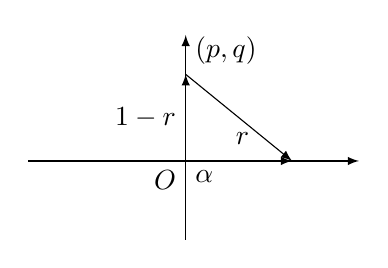
\begin{tikzpicture}[baseline=(current bounding box.center),x=1.0cm,y=1.0cm,>=latex]
\draw[->] (-2.0,0) -- (2.2,0);
\draw[->] (0,-1.0) -- (0,1.6);
\node[below left] at (0,0) {$O$};
\node[below right] at (0,0) {$\alpha$};
\draw[->] (0,0) -- (0,1.1);
\draw[->] (0,1.1) -- (1.35,0);
\draw[->] (0,0) -- (1.35,0);
\node[above right] at (0,1.1) {$(p,q)$};
\node[left] at (0,0.55) {$1-r$};
\node[above] at (.72,0.08) {$r$};
\end{tikzpicture}
\]
\[
B_r^{pq}(X_\alpha)=B_{r+1}^{pq}(X_\alpha)\quad\text{当 }r>p,
\]
\[
Z_r^{pq}(X_\alpha)=Z_{r+1}^{pq}(X_\alpha)\quad\text{当 }r>\alpha-p.
\]

c) 当 \(X\) 满足 Mittag-Leffler 条件时, 各投射系 \(\gr^p(X)\) 本质常值 (EGA \(0_{\mathrm{III}}\) 13.4.3). 立即得到: 对 \(r<+\infty\), 各投射系 \(E_r^{pq}(X)\) 本质常值. 用
\[
\mathcal E_r^{pq}(X)
\]
表示其投射极限. 由于微分算子可取极限, 这样得到谱滤子 \(\mathcal E_r^{pq}(X)\), \(p,q\in\mathbb Z,\ r\ge1\). 与此谱滤子相伴的对象
\[
\mathcal Z_r^{pq}(X),\quad \mathcal B_r^{pq}(X)\quad(r<+\infty)
\]
恰为本质常值投射系 \(Z_r^{pq}(X)\) 与 \(B_r^{pq}(X)\) 的极限.

由 b) 还得
\[
B_\infty^{pq}(X)=B_{p+1}^{pq}(X),
\]
因此可置
\[
\mathcal B_\infty^{pq}(X)=\mathcal B_{p+1}^{pq}(X).
\]
仍假设 \(X\) 满足 (ML). 由于对每个 \(\alpha\),
\[
B_r^{pq}(X_\alpha)=B_{r+1}^{pq}(X_\alpha)\qquad(r>p),
\]
故有一列典范单态射
\begin{equation}
\cdots\subset\mathcal E_r^{pq}(X)\subset\cdots\subset\mathcal E_{p+2}^{pq}(X)\subset\mathcal E_{p+1}^{pq}(X).
\tag{S}
\end{equation}
此后假设 \(X\) 严格. \(Z_r^{pq}(X_n)\) 与 \(B_r^{pq}(X_n)\) 的下述表达式:
\[
B_r^{pq}(X_n)=
\Im\!\left[
T^{p+q-1}\bigl(F^{p-r+1}X_n/F^pX_n\bigr)
\xrightarrow{\partial}
T^{p+q}\bigl(F^pX_n/F^{p+1}X_n\bigr)
\right],
\]
\[
Z_r^{pq}(X_n)=
\Im\!\left[
T^{p+q}\bigl(F^pX_n/F^{p+r}X_n\bigr)
\longrightarrow
T^{p+q}\bigl(F^pX_n/F^{p+1}X_n\bigr)
\right],
\]
表明
\begin{equation}
\left\{
\begin{array}{ll}
B_r^{pq}(X_m)\xrightarrow{\sim}B_r^{pq}(X_n)&\text{当 }m\ge n\ge p,\\[3pt]
Z_r^{pq}(X_m)\xrightarrow{\sim}Z_r^{pq}(X_n)&\text{当 }m\ge n\ge p+r-1,
\end{array}
\right.
\tag{\(d_1\)}
\end{equation}
其中典范态射均为同构. 特别地, 典范态射
\[
\mathcal E_r^{pq}(X)\longrightarrow E_r^{pq}(X_{p+r-1})
\]
为同构. 此外, 由 b) 得
\begin{equation}
\left\{
\begin{array}{ll}
Z_\infty^{pq}(X_{p+r-1})=Z_r^{pq}(X_{p+r-1})&(r\ge1),\\[3pt]
B_\infty^{pq}(X_{p+r-1})=B_r^{pq}(X_{p+r-1})&(r>p).
\end{array}
\right.
\tag{\(d_2\)}
\end{equation}
由此对每个 \(r\) 可以定义典范满态射
\[
\theta_r^{pq}:\mathcal E_r^{pq}(X)\longrightarrow E_\infty^{pq}(X_{p+r-1})
\]
当 \(r>p\) 时它是同构. 再者, 若整数 \(a\) 满足
\[
\mathcal B_r^{pq}(X)=\mathcal B_a^{pq}(X)\qquad(r\ge a),
\]
例如取 \(a=p+1\) 即可, 因而有
\begin{equation}
\cdots\hookrightarrow\mathcal E_r^{pq}(X)\hookrightarrow\cdots\hookrightarrow
\mathcal E_{a+1}^{pq}(X)\hookrightarrow\mathcal E_a^{pq}(X),
\tag{S bis}
\end{equation}
则对 \(s\ge r\ge a\), 图
\begin{equation}
\begin{array}{ccc}
\mathcal E_s^{pq}(X)&\xrightarrow[\epi]{\theta_s^{pq}}&E_\infty^{pq}(X_{p+s-1})\\
\downarrow&&\downarrow\can\\
\mathcal E_r^{pq}(X)&\xrightarrow[\epi]{\theta_r^{pq}}&E_\infty^{pq}(X_{p+r-1})
\end{array}
\tag{\(d_3\)}
\end{equation}
交换.

\subsubsection*{A.3. Shih 定理的一个变式}
设给定按理想 \(F^i(S)\), \(i\ge0\), 滤过的环 \(S\), 它作用于 \(X\), 且与 \(X\) 作为投射系的滤过相容.

由 A.1 的一般论述, 对每个整数 \(i\), \(\gr^i(S)\) 以双次数 \((i,-i)\) 的态射作用于双分次对象 \(E_r(X)\). 特别地, 对每个整数 \(n\),
\[
E_r^{(n)}(X)=\bigl(E_r^{p,q}(X)\bigr)_{p+q=n}
\]
典范地具有分次 \((\gr^\bullet(S),\mathcal D)\) 模结构. 取极限后, 对
\[
\mathcal E_r^{(n)}(X)=\bigl(\mathcal E_r^{p,q}(X)\bigr)_{p+q=n}.
\]
亦然. 环 \(S\) 作用于 \(X\), 且与其作为投射系的滤过相容, 因而也作用于每个整数 \(n\) 对应的 \(T^n(X)\). 所以严格相伴分次对象 \(\grs(X)\) 典范地具有分次 \((\gr^\bullet(S),\mathcal C)\) 模结构; 同样, 当 \(T^n(X)\) 满足 (ML) 时, 严格相伴分次对象 \(\grs\,T^n(X)\) 典范地具有分次 \((\gr^\bullet(S),\mathcal D)\) 模结构.

\begin{statement}{定理 A.3}
假设对某个整数 \(n\), 分次 \((\gr^\bullet(S),\mathcal D)\) 模
\[
\mathcal E_1^{(n)}(X)=T^n(\grs^\bullet X)
\quad\text{与}\quad
\mathcal E_1^{(n-1)}(X)=T^{n-1}(\grs^\bullet X)
\]
均为诺特的. 则:
\begin{enumerate}[label=\textup{(\roman*)}]
\item \(T^n(X)\) 满足 (MLAR);
\item \(\grs\,T^n(X)\) 是诺特 \((\gr^\bullet(S),\mathcal D)\) 模.
\end{enumerate}
\end{statement}

\begin{prooftext}
i) 对每对整数 \((m,r)\),
\[
\mathcal B_r^{(m)}(X)=\bigl(\mathcal B_r^{p,m-p}(X)\bigr)_{p\in\mathbb N}
\]
是 \(\mathcal E_1^{(m)}(X)\) 的分次 \((\gr^\bullet(S),\mathcal D)\) 子模. 特别地, 对每个整数 \(m\), 各 \(\mathcal B_r^{(m)}(X)\) 构成以 \(r\) 为指标的 \(\mathcal E_1^{(m)}(X)\) 的分次 \((\gr^\bullet(S),\mathcal D)\) 子模的递增序列. 利用 \(\mathcal E_1^{(n)}(X)\) 与 \(\mathcal E_1^{(n-1)}(X)\) 是诺特分次 \((\gr^\bullet(S),\mathcal D)\) 模这一事实, 得到序列
\[
\bigl[\mathcal B_r^{(n)}(X)\bigr]_{r\in\mathbb N}
\qquad\text{与}\qquad
\bigl[\mathcal B_r^{(n-1)}(X)\bigr]_{r\in\mathbb N}
\]
稳定.

所以存在整数 \(a\ge1\), 使对每个满足 \(p+q=n\) 或 \(n-1\) 的 \((p,q)\), 有
\begin{equation}
\mathcal B_r^{pq}(X)=\mathcal B_a^{pq}(X)\qquad(r\ge a).
\tag{A.3.1}
\end{equation}
因此当 \(r\ge a+1\) 时, 以 \(\mathcal E_r^{pq}(X)\), \(p+q=n\), 为源或目标的箭头 \(d_r\) 均为零. 换言之, 由 (A.3.1) 在 \(p+q=n\) 时得到的单态射
\[
\mathcal E_s^{pq}(X)\hookrightarrow\mathcal E_r^{pq}(X)\qquad(s\ge r\ge a+1)
\]
实际上是同构. 对 \(s\ge r\ge a+1\), 图 \((d_3)\) 在 \(p+q=n\) 时的交换性
\[
\begin{array}{ccc}
\mathcal E_s^{pq}(X)&\xrightarrow[\epi]{\theta_s^{pq}}&E_\infty^{pq}(X_{p+s-1})\\
\downarrow\sim&&\downarrow\\
\mathcal E_r^{pq}(X)&\xrightarrow[\epi]{\theta_r^{pq}}&E_\infty^{pq}(X_{p+r-1})
\end{array}
\]
表明转移态射
\[
E_\infty^{pq}(X_{p+s-1})\longrightarrow E_\infty^{pq}(X_{p+r-1}),
\]
为满态射, 而它总是单态射 (参见 a)), 因而是同构. 换言之, 投射系
\[
r\longmapsto\left[\bigoplus_p\gr^p T^n(X_{p+r})\right]_{r\ge1}
\]
从 \(r=a\) 起为常值, 所以由 (4.1.3), \(T^n(X)\) 满足 (MLAR).

ii) 用
\[
\mathcal E_\infty^{(n)}(X),\quad
\mathcal Z_\infty^{(n)}(X),\quad
\mathcal B_\infty^{(n)}(X)
\]
表示上面所考虑的各个以 \(r\) 为指标的投射系的``极限'', 则看到
\[
\mathcal E_\infty^{(n)}(X)=
\mathcal Z_\infty^{(n)}(X)/\mathcal B_\infty^{(n)}(X)
\]
是诺特 \((\gr^\bullet(S),\mathcal D)\) 模, 因为 \(\mathcal Z_\infty^{(n)}(X)\) 包含于 \(\mathcal E_1^{(n)}(X)\). 此外, 由 A.2 a) 得
\[
\mathcal E_\infty^{(n)}(X)=\grs\,T^n(X).
\]
\end{prooftext}

\clearpage\phantomsection\addcontentsline{toc}{section}{\texorpdfstring{报告 VI --- $\ell$ 进上同调}{报告 VI --- ℓ 进上同调}}
\section*{报告 VI}

\begin{center}
\textbf{\(\ell\) 进上同调}\\[0.5em]
J.-P. Jouanolou 著
\end{center}

本报告始终固定素数 \(\ell\).

照例, \(X_{\mathrm{\acute et}}\) 表示预概形 \(X\) 的平展景.

\subsection*{1. 可构造 \(\ell\) 进层}

本节始终固定一个局部诺特预概形 \(X\).

\subsubsection*{1.1. 定义与一般论述}

\begin{statement}{定义 1.1.1}
\(X\) 上的可构造 \(\ell\) 进层是 \(X_{\mathrm{\acute et}}\) 上可构造阿贝尔层的一个 \((\ell\mathbb Z)\) 进投射系 (V 3.1.1).
\end{statement}

要使 \(X_{\mathrm{\acute et}}\) 上阿贝尔层的 \((\ell\mathbb Z)\) 进投射系
\[
F=(F_n)_{n\in\mathbb N}
\]
成为可构造 \(\ell\) 进层, 只须 \(F_0\) 可构造. 事实上, 该断言是局部的, 而在诺特情形由 (V 5.1.2) 得出.

用 \(\Abc(X)\) 表示 \(X\) 上的可构造阿贝尔层范畴. 用
\[
\ell\text{-}\adc(X)
\]
表示 \(\Hom(\mathbb N^\circ,\Abc(X))\) 中由可构造 \(\ell\) 进层生成的满子范畴. 沿用报告 V 的记号,
\[
\ell\text{-}\adc(X)=(\ell\mathbb Z)\text{-}\ad(\Abc(X)).
\]
用 \(\Ab(X)\) 表示 \(X_{\mathrm{\acute et}}\) 上的阿贝尔层范畴. 已知 (SGA 4 IX 2.9), 当 \(X\) 为诺特的时, \(X\) 上的可构造阿贝尔层就是诺特阿贝尔层. 此时范畴 \(\ell\text{-}\adc(X)\) 显然可等同于报告 V 中记为
\[
(\ell\mathbb Z)\text{-}\adn(\Ab(X))
\]
的范畴.

\begin{statement}{命题 1.1.2}
设 \(F=(F_n)_{n\in\mathbb N}\) 为范畴 \(\Hom(\mathbb N^\circ,\Ab(X))\) 的对象. \(F\) 为可构造 \(\ell\) 进的充要条件是: 它对于 \(X\) 的平展拓扑局部地具有此性质.
\end{statement}

\begin{prooftext}[证明]
显然, \(F\) 为 \(\ell\) 进的这一性质可在景的终对象的一个覆盖上判定. 此外, 由 (SGA 4 IX 2.8), 若各 \(F_n\) 局部可构造, 则它们可构造.
\end{prooftext}

\begin{statement}{命题 1.1.3}
\(X\) 上可构造 \(\ell\) 进层的范畴 \(\ell\text{-}\adc(X)\) 为阿贝尔范畴. 当 \(X\) 为诺特的时, 该范畴为诺特的.
\end{statement}

\begin{prooftext}[证明]
当 \(X\) 为诺特的时, 这两个断言都是 (V 5.2.3) 的推论. 一般情形下, 须说明 \(X\) 上可构造 \(\ell\) 进层的每个态射
\[
u:F\longrightarrow G
\]
都有核与余核.

对于余核, 这由 (V 3.1.3) 得出. 现证明 \(u\) 的核存在. 对 \(X\) 的每个诺特开集 \(V\), 已知 \(u\) 在 \(V\) 上的限制
\[
u_V:F_V\longrightarrow G_V,
\]
在范畴 \(\ell\text{-}\adc(V)\) 中有核, 且有如下简单描述. 若 \(K\) 为 \(u_V\) 在范畴 \(\Hom(\mathbb N^\circ,\Ab(V))\) 中的核, 则 \(K\) 满足 Mittag-Leffler-Artin-Rees 条件; 用 \(K'\) 表示其普遍像所成投射系, 则存在整数 \(r\), 使投射系
\[
m_r(K')=\bigl(K'_{n+r}/\ell^{\,n+1}K'_{n+r}\bigr)_{n\in\mathbb N}
\]
(配以显然的转移态射) 为可构造 \(\ell\) 进的. 下述显然的复合是 \(u_V\) 在范畴 \(\ell\text{-}\adc(V)\) 中的核:
\[
m_r(K')\longrightarrow K'\longrightarrow K.
\]
上述构造特别表明: 若 \(W\) 为包含于 \(V\) 的开集, 则 \(u_V\) 的核在 \(W\) 上的限制是 \(u_W\) 的核. 设 \((V_i)_{i\in I}\) 为 \(X\) 的诺特开覆盖. 若 \(i,j\) 为 \(I\) 的两个元素, 则 \(u_{V_i}\) 与 \(u_{V_j}\) 的核在 \(V_i\cap V_j\) 上的限制典范同构, 因而可将它们粘合, 构造 \(u\) 的核.
\end{prooftext}

\subsubsection*{1.1.4}
设 \(F=(F_n)_{n\in\mathbb N}\) 为可构造 \(\ell\) 进层. 由于环 \(\mathbb Z_\ell\) 显然作用于每个层 \(F_n\), 它也作用于 \(F\). 此外, 若 \(F,G\) 为两个可构造 \(\ell\) 进层, 且
\[
u:F\longrightarrow G
\]
为态射, 则 \(u\) 与 \(\mathbb Z_\ell\) 分别在 \(F,G\) 上的作用相容. 这表明 \(\ell\text{-}\adc(X)\) 典范地具有阿贝尔 \(\mathbb Z_\ell\) 范畴结构.

因此可使用下述术语.

\begin{statement}{术语}
下文将可构造 \(\ell\) 进层称为可构造 \(\mathbb Z_\ell\) 层.
\end{statement}

应注意不要将这一概念与 \((\mathbb Z_\ell)_X\) 模的概念混淆; 后者在下文中不会使用.

范畴 \(\ell\text{-}\adc(X)\) 也记为
\[
\mathbb Z_\ell\text{-}\fc(X).
\]

\subsubsection*{1.2. 可构造扭常值 \(\mathbb Z_\ell\) 层}

\begin{statement}{定义 1.2.1}
可构造 \(\mathbb Z_\ell\) 层
\[
F=(F_n)_{n\in\mathbb N}
\]
称为扭常值的, 当且仅当各层 \(F_n\) 在 \(X_{\mathrm{\acute et}}\) 上局部常值.
\end{statement}

可构造扭常值 \(\mathbb Z_\ell\) 层范畴是 \(\mathbb Z_\ell\text{-}\fc(X)\) 中由可构造扭常值 \(\mathbb Z_\ell\) 层生成的满子范畴.

\begin{statement}{例 1.2.2}
\(\mathbb Z_\ell\) 层 \(\mathbb Z_\ell(1)\).
\end{statement}

假设整数 \(\ell\) 与 \(X\) 的剩余特征互素. 对每个整数 \(n\), 取 \(\ell\) 次幂定义局部常值层的态射:
\[
\mu_{\ell^{n+1}}\longrightarrow \mu_{\ell^n}.
\]
这显然定义一个投射系:
\[
\mathbb Z_\ell(1)=(\mu_{\ell^{n+1}})_{n\in\mathbb N}.
\]
对每个整数 \(n\), 归约到 \(\mu_{\ell^n}\) 与 \(\mu_{\ell^{n+1}}\) 均为常值的情形, 即可看到投射系 \(\mathbb Z_\ell(1)\) 为 \(\ell\) 进的.

当 \(X=\Spec(K)\), 其中 \(K\) 是素域的有限型扩域时, \(\mathbb Z_\ell\) 层 \(\mathbb Z_\ell(1)\) 给出一个可构造扭常值 \(\ell\) 进层 (1.2.1) 的例子: 不存在 \(K\) 的有限平展扩张 \(K'\), 使各 \(F_n\) 在 \(X'=\Spec(K')\) 上的逆像为常值. 事实上, \(K'\) 必须对每个整数 \(n\) 都包含一个本原 \(\ell^n\) 次单位根, 而素域的有限型扩域不可能具有此性质.

\begin{statement}{回顾 1.2.3}
(SGA 1 V 7). 已知预概形 \(T\) 上可构造局部常值阿贝尔挠层的范畴, 等价于赋予阿贝尔 \(X\) 群结构的 \(T\) 的平展覆盖的范畴.
\end{statement}

现设 \(X\) 为连通局部诺特预概形. 用 \(R_X\) 表示 \(X\) 的平展覆盖范畴, 用 \(\Ensf\) 表示有限集合范畴. 若 \(a\) 为 \(X\) 的几何点, 则令 \(F_a\) 为函子
\[
F_a:R_X\longrightarrow \Ensf,
\]
它给 \(X\) 的每个平展覆盖配上其在 \(a\) 处的几何纤维. \(X\) 在 \(a\) 处的基本群
\[
\pi_1(X)=\pi_1(X,a)
\]
按定义为赋予适当拓扑的 \(F_a\) 的自同构群, 因此可将函子 \(F_a\) 解释为函子
\[
R_X\longrightarrow \Ensf(\pi_1)
\]
即从范畴 \(R_X\) 到赋予 \(\pi_1=\pi_1(X,a)\) 的连续作用的有限集合范畴的函子.

回顾下述命题.

\begin{statement}{命题 1.2.3.1}
函子
\[
F_a:R_X\longrightarrow \Ensf(\pi_1)
\]
是范畴等价. 它与归纳极限和有限投射极限交换.
\end{statement}

用 \(Lc(X)\) 与 \(\Abf(\pi_1)\) 分别表示可构造局部常值阿贝尔挠层范畴, 以及赋予基本群连续作用的有限阿贝尔群范畴. 函子 \(F_a\) 诱导正合函子, 仍记为 \(F_a\),
\[
F_a:Lc(X)\longrightarrow \Abf(\pi_1),
\]
它是范畴等价.

\subsubsection*{1.2.4. 连通预概形上的扭常值 \(\mathbb Z_\ell\) 层}

(1.2.3) 的回顾立即给出下述引理.

\begin{statement}{引理 1.2.4.1}
将 \(F_a\) 延拓到以 \(\mathbb N\) 为指标的投射系范畴所得的 \(\widehat F_a\), 诱导从可构造扭常值 \(\ell\) 进层范畴到下述范畴的等价:
\[
(\ell\mathbb Z)\text{-}\ad(\Abf(\pi_1)).
\]
\end{statement}

现设 \(F=(F_n)_{n\in\mathbb N}\) 为范畴
\[
(\ell\mathbb Z)\text{-}\ad(\Abf(\pi_1)).
\]
的对象. 其投射极限
\[
\varprojlim_{\mathbb N}F_n
\]
自然具有有限型 \(\mathbb Z_\ell\) 模结构, 且 \(\pi_1\) 对于 \(\ell\) 进拓扑连续地作用于其上. 回忆, 若 \(G,M\) 分别表示投有限群与有限型 \(\mathbb Z_\ell\) 模, 则 \(G\) 在 \(M\) 上的连续作用指连续映射
\[
G\times M\longrightarrow M,\qquad (g,m)\longmapsto g\cdot m,
\]
满足
\[
\text{(i)}\quad g\cdot(m+n)=g\cdot m+g\cdot n\quad (g\in G,\ m,n\in M),
\]
及
\[
\text{(ii)}\quad (gh)\cdot m=g\cdot(h\cdot m)\quad (g,h\in G,\ m\in M).
\]
此时显然, 对每个 \(\ell\) 进整数 \(a\),
\[
g\cdot(am)=a(g\cdot m)\qquad (g\in G,\ m\in M).
\]
此外, 从 \(M\) 到 \(M\) 的可逆 \(\mathbb Z_\ell\) 线性映射所成的群, 记为 \(\GL(M)\), 可等同于各群 \(\GL(M/\ell^{n+1}M)\) 的投射极限. 因为这些群有限, 群 \(\GL(M)\) 自然具有投有限群结构, 特别具有紧拓扑群结构. 容易验证, 给定投有限群 \(G\) 在 \(M\) 上的连续作用, 等价于给定拓扑群态射
\[
G\longrightarrow \GL(M),
\]
其中后一个群赋予刚才描述的拓扑. 在此基础上, 显然可定义函子
\[
\varprojlim_{\mathbb N}:(\ell\mathbb Z)\text{-}\ad(\Abf(\pi_1))\longrightarrow
\mathbb Z_\ell\text{-}\modn(\pi_1),
\]
其中 \(\mathbb Z_\ell\text{-}\modn(\pi_1)\) 表示赋予 \(\pi_1\) 的连续作用的有限型 \(\mathbb Z_\ell\) 模范畴.

于是可陈述下述引理.

\begin{statement}{引理 1.2.4.2}
上述函子
\[
\varprojlim_{\mathbb N}:(\ell\mathbb Z)\text{-}\ad(\Abf(\pi_1))
\longrightarrow \mathbb Z_\ell\text{-}\modn(\pi_1)
\]
是范畴等价.
\end{statement}

\begin{prooftext}[证明]
它显然本质满: 赋予 \(\pi_1\) 连续作用的有限型 \(\mathbb Z_\ell\) 模 \(E\), 是投射系
\[
(E/\ell^{n+1}E)_{n\in\mathbb N},
\]
的像, 其中配以显然的 \(\pi_1\) 作用. 现设
\[
F=(F_n)_{n\in\mathbb N},\qquad G=(G_n)_{n\in\mathbb N}
\]
为范畴 \((\ell\mathbb Z)\text{-}\ad(\Abf(\pi_1))\) 的两个对象; 为简便, 用 \(\Hom_{\pi_1}(F,G)\) 表示该范畴中从 \(F\) 到 \(G\) 的态射集. 忘掉 \(\pi_1\) 的作用, 可将 \(F,G\) 视为有限阿贝尔群的 \(\ell\) 进投射系范畴中的对象, 并用 \(\Hom_0(F,G)\) 表示这一范畴中从 \(F\) 到 \(G\) 的态射集. 群 \(\pi_1\) 以下述方式作用于 \(\Hom_0(F,G)\): \(\pi_1\) 的元素 \(s\) 显然在有限阿贝尔群的 \(\ell\) 进投射系范畴中, 分别定义 \(F,G\) 的两个自同构, 仍用同一记号表示; 若 \(u\) 属于 \(\Hom_0(F,G)\), 置
\[
s\cdot u=sus^{-1}.
\]
此时显然, \(\Hom_{\pi_1}(F,G)\) 典范地等同于 \(\Hom_0(F,G)\) 中的 \(\pi_1\) 不变元集合; 同样, 对每个 \(n\), \(\Hom_{\pi_1}(F_n,G_n)\) 等同于
\[
\Hom_{\mathbb Z}(F_n,G_n)^{\pi_1},
\]
其中 \(\pi_1\) 的作用按类似方式定义. 例如由 (Serre, Groupes proalgébriques, 命题 12), 若用 \(M,N\) 分别表示 \(F,G\) 的投射极限, 则有
\[
\Hom_{\mathbb Z_\ell}(M,N)=\varprojlim_n\Hom_{\mathbb Z}(F_n,G_n).
\]
对两边取 \(\pi_1\) 不变元, 并利用这一操作由投射极限给出、因而与投射极限交换这一事实, 即得断言.
\end{prooftext}

引理 1.2.4.1 和 1.2.4.2 给出下述较不精确的命题.

\begin{statement}{命题 1.2.5}
连通局部诺特预概形 \(X\) 上可构造扭常值 \(\mathbb Z_\ell\) 层的范畴, 等价于赋予 \(\pi_1(X)\) 对于 \(\ell\) 进拓扑的连续作用的有限型 \(\mathbb Z_\ell\) 模范畴.
\end{statement}

\begin{statement}{注}
设 \(F\) 为可构造扭常值 \(\mathbb Z_\ell\) 层, \(M\) 为对应的、赋予 \(\pi_1\) 连续作用的有限型 \(\mathbb Z_\ell\) 模. 要使 \(F\) 局部常值, 显然只须 \(\pi_1\) 经一个有限商作用于 \(M\); 这并非总成立 (1.2.2). 当 \(X\) 正规时, 这一条件也是必要的. 为说明这一点, 将 \(X\) 分解为连通分支后, 可归约到 \(X\) 整的情形. 断言此时若 \(K\) 表示其有理函数域, 且存在 \(K\) 的有限可分扩张 \(K'\), 使 \(F\) 在 \(\Spec(K')\) 上的逆像 \(F_{K'}\) 为常值, 则群 \(\pi_1(X)\) 经一个有限群作用于 \(M\). 事实上 (SGA 1 V 8.2), \(\pi_1(K)\to\pi_1(X)\) 满射, 而假设意味着复合
\[
\pi_1(K)\longrightarrow \pi_1(X)\longrightarrow \Aut(M)
\]
的核具有有限指数. 因而 \(\pi_1(X)\to\Aut(M)\) 的核也具有有限指数.
\end{statement}

\begin{statement}{命题 1.2.6}
设 \(X\) 为局部诺特预概形, \(F\) 为 \(X_{\mathrm{\acute et}}\) 上以 \(\mathbb N\) 为指标的阿贝尔层投射系. 下述断言等价:
\begin{enumerate}[label=(\roman*)]
\item \(F\) 为可构造 \(\mathbb Z_\ell\) 层;
\item \(X\) 的每个诺特开集 \(U\) 都是有限个局部闭子集 \((Z_i)_{1\le i\le q}\) 的并, 且 \(F\) 在这些子集上的逆像是可构造扭常值 \(\mathbb Z_\ell\) 层;
\item \(X\) 有一个开覆盖, 其每个开集是有限个局部闭子集的并, 且 \(F\) 在这些子集上的逆像是可构造扭常值 \(\mathbb Z_\ell\) 层.
\end{enumerate}
\end{statement}

\begin{prooftext}[证明]
显然 (ii) 蕴含 (iii).

(iii) \(\Longrightarrow\) (i): 若 \(F\) 满足 (iii), 则其几何纤维为 \(\ell\) 进的, 因而由 (SGA 4 VIII 3.6), \(F\) 为 \(\ell\) 进的. 此外, 其分量可构造 (SGA 4 IX 2.8).

为说明 (i) 蕴含 (ii), 立即归约到 \(X\) 为诺特的情形. 若 \(F\) 为可构造 \(\ell\) 进的, 则其严格分次对象 \(\operatorname{gr}^s(F)\) 是诺特 \((\operatorname{gr}_\ell\mathbb Z,\Ab(X))\) 模 (V 5.1.6). 因而 (SGA 4 IX 2.9), \(X\) 是有限个局部闭子集 \((Z_i)_{1\le i\le q}\) 的并, 且 \(\operatorname{gr}^s(F)\) 在这些子集上的逆像是局部常值层. 由于对有限纤维的层, 局部常值性对于扩张稳定, 可得对每个整数 \(n\), \(F\) 的分量 \(F_n\) 在每个 \(Z_i\) 上的逆像均为局部常值层.
\end{prooftext}

\subsubsection*{1.3. \(\mathbb Z_\ell\) 层上的运算 \(\otimes\) 与 \(\Hom\)}

\paragraph{1.3.1. 张量积.}
设 \(F,G\) 为范畴 \(\Hom(\mathbb N^\circ,\Ab(X))\) 的两个对象. 若
\[
F=(F_n)_{n\in\mathbb N}\quad\text{且}\quad G=(G_n)_{n\in\mathbb N},
\]
则 \(F,G\) 的张量积 \(F\otimes G\) 在对象上由下式定义, 在箭头上按显然方式定义:
\[
(F\otimes G)_n=F_n\otimes G_n.
\]
更准确地说, 显然可定义一个右正合加性双函子, 称为张量积:
\[
\otimes:\Hom(\mathbb N^\circ,\Ab(X))\times \Hom(\mathbb N^\circ,\Ab(X))
\longrightarrow \Hom(\mathbb N^\circ,\Ab(X)).
\]

\begin{statement}{命题 1.3.2}
若 \(F,G\) 为两个可构造 \(\mathbb Z_\ell\) 层, 则张量积 \(F\otimes G\) 为可构造 \(\mathbb Z_\ell\) 层.
\end{statement}

\begin{prooftext}[证明]
\(\ell\) 进性显然. 此外, 由可构造层的定义 (SGA 4 IX 2.3) 立即得到, 两个可构造层的张量积可构造.
\end{prooftext}

因此通过限制, 定义一个右正合加性双函子, 仍称为张量积:
\[
\otimes:\mathbb Z_\ell\text{-}\fc(X)\times \mathbb Z_\ell\text{-}\fc(X)
\longrightarrow \mathbb Z_\ell\text{-}\fc(X).
\]

\subsubsection*{1.3.3. 同态层}

设 \(F=(F_n)_{n\in\mathbb N}\) 与 \(G=(G_n)_{n\in\mathbb N}\) 为两个可构造 \(\mathbb Z_\ell\) 层. 假设 \(F\) 局部自由, 即对每个整数 \(n\), 层 \(F_n\) 在常值层
\[
(\mathbb Z/\ell^{\,n+1}\mathbb Z)_X.
\]
上局部自由. 对每个整数 \(n\), 结构正合列
\[
G_{n+1}\xrightarrow{\ell^{\,n+1}}G_{n+1}\longrightarrow G_n\longrightarrow 0
\]
由于 \(F_{n+1}\) 在 \((\mathbb Z/\ell^{\,n+2}\mathbb Z)_X\) 上局部自由, 给出正合列
\[
\cHom(F_{n+1},G_{n+1})
 \xrightarrow{\ell^{\,n+1}}
\cHom(F_{n+1},G_{n+1})
 \longrightarrow
\cHom(F_{n+1},G_n)
 \longrightarrow 0.
\tag{1}
\]
由于 \(\ell^{\,n+1}G_n=0\), 结构正合列
\[
F_{n+1}\xrightarrow{\ell^{\,n+1}}F_{n+1}\longrightarrow F_n\longrightarrow 0
\]
显然定义一个同构
\[
\cHom(F_{n+1},G_n)\xleftarrow{\sim}\cHom(F_n,G_n).
\tag{2}
\]
结合 (1) 和 (2), 对每个整数 \(n\) 得到态射
\[
\cHom(F_{n+1},G_{n+1})\longrightarrow \cHom(F_n,G_n).
\]
从而得到投射系
\[
\cHom(F,G)=\bigl(\cHom(F_n,G_n)\bigr)_{n\in\mathbb N},
\]
它显然是一个 \(\mathbb Z_\ell\) 层.

\subsubsection*{1.3.4. 可逆 \(\ell\) 进层的一般论述. 对层 \(\mathbb Z_\ell(r)\) (\(r\in\mathbb Z\)) 的应用}

设 \(L\) 为可构造 \(\mathbb Z_\ell\) 层. 若对每个整数 \(n\), 其第 \(n\) 个分量 \(L_n\) 是可逆 \((\mathbb Z/\ell^{\,n+1}\mathbb Z)_X\) 模, 即秩一局部自由模, 则称 \(L\) 可逆. 这等价于: \(L\) 在上小节的意义下局部自由, 且各 \(L_n\) 的几何纤维是非零循环阿贝尔群.

若 \(L\) 为可逆 \(\mathbb Z_\ell\) 层, 约定置
\[
L^{-1}=\cHom(L,\mathbb Z_\ell).
\]
显然有同构
\[
L\otimes L^{-1}\xrightarrow{\sim}\mathbb Z_\ell,
\]
它逐分量由类似同构 (EGA \(0_I\) 5.4.3.1) 得到. 按照 (EGA \(0_I\) 5.4.4), 约定置 \(L^{\otimes0}=\mathbb Z_\ell\), 并对 \(n\ge1\) 置
\[
L^{\otimes -n}=(L^{-1})^{\otimes n}.
\]
在此记号下, 对所有有理整数 \(m,n\), 有典范函子性同构
\[
L^{\otimes m}\otimes L^{\otimes n}\xrightarrow{\sim}L^{\otimes(m+n)}
\]
此外, 该同构具有通常的结合性.

特别地, 分次对象
\[
(L^{\otimes i})_{i\in\mathbb N}\quad\text{与}\quad(L^{\otimes i})_{i\in\mathbb Z}
\]
为分别按 \(\mathbb N\) 与 \(\mathbb Z\) 分次的 \(\mathbb Z_\ell\) 代数.

\begin{statement}{例}
(1.2.2) 中定义的 \(\mathbb Z_\ell\) 层 \(\mathbb Z_\ell(1)\) 可逆, 下文约定置
\[
\mathbb Z_\ell(r)=\bigl(\mathbb Z_\ell(1)\bigr)^{\otimes r}\qquad (r\in\mathbb Z).
\]
\end{statement}

\subsubsection*{1.4. 从可构造 \(\mathbb Z_\ell\) 层范畴构造的各种范畴}

\paragraph{1.4.1. 可构造 \(A\) 层 (\(A\) 为有限 \(\mathbb Z_\ell\) 代数).}
设 \(A\) 为有限 \(\mathbb Z_\ell\) 代数. 按如下方式定义范畴, 记为
\[
A\text{-}\fc(X),
\]
其对象称为可构造 \(A\) 层.

\begin{enumerate}[label=(\roman*)]
\item \(A\text{-}\fc(X)\) 的对象为二元组 \((F,u)\), 其中 \(F\) 为可构造 \(\mathbb Z_\ell\) 层, 而 \(u\) 为 \(\mathbb Z_\ell\) 代数态射
\[
u:A\longrightarrow \End(F).
\]
\item 若 \((F,u),(F',u')\) 为两个可构造 \(A\) 层, 则箭头 \((F,u)\to(F',u')\) 是 \(\mathbb Z_\ell\) 层的态射
\[
f:F\longrightarrow F'
\]
使得对 \(A\) 的每个元素 \(a\), 下图交换:
\[
\begin{tikzcd}
F \arrow[r,"f"] \arrow[d,"u(a)"'] & F' \arrow[d,"u'(a)"]\\
F \arrow[r,"f"'] & F'.
\end{tikzcd}
\]
\end{enumerate}

可构造扭常值 \(A\) 层是底层可构造 \(\mathbb Z_\ell\) 层为扭常值的可构造 \(A\) 层. 可构造扭常值 \(A\) 层范畴是可构造 \(A\) 层范畴中由可构造扭常值 \(A\) 层生成的满子范畴.

由 (1.2.4) 立即得到: 若 \(X\) 连通, 则可构造扭常值 \(A\) 层范畴等价于赋予 \(\pi_1(X)\) 的连续 \(A\) 线性作用的有限型 \(A\) 模范畴; 连续性是对于底层有限型 \(\mathbb Z_\ell\) 模而言的 (1.2.4).

\paragraph{1.4.2. 可构造 \(\mathbb Q_\ell\) 层.}
显然, \(\mathbb Z_\ell\text{-}\fc(X)\) 中由可构造挠 \(\mathbb Z_\ell\) 层, 即被 \(\ell\) 的某个幂消去的层, 生成的满子范畴是厚的.

\begin{statement}{定义 1.4.3}
\(X\) 上可构造 \(\mathbb Q_\ell\) 层范畴, 记为
\[
\mathbb Q_\ell\text{-}\fc(X),
\]
是 Gabriel 博士论文意义下的商阿贝尔范畴: 以 \(\mathbb Z_\ell\text{-}\fc(X)\) 模去挠 \(\mathbb Z_\ell\) 层所成的厚阿贝尔子范畴. \(\mathbb Q_\ell\text{-}\fc(X)\) 的对象称为可构造 \(\mathbb Q_\ell\) 层.
\end{statement}

范畴 \(\mathbb Q_\ell\text{-}\fc(X)\) 有如下简单描述. 其对象集与 \(\mathbb Z_\ell\text{-}\fc(X)\) 相同, 且若 \(F,G\) 为两个这样的对象, 则
\[
\Hom_{\mathbb Q_\ell}(F,G)
=\mathbb Q_\ell\otimes_{\mathbb Z_\ell}\Hom_{\mathbb Z_\ell}(F,G),
\]
其中 \(\Hom_{\mathbb Z_\ell}(F,G)\) 与 \(\Hom_{\mathbb Q_\ell}(F,G)\) 分别表示 \(\mathbb Z_\ell\text{-}\fc(X)\) 与 \(\mathbb Q_\ell\text{-}\fc(X)\) 中的态射. 事实上, 若
\[
u:\mathbb Z_\ell\text{-}\fc(X)\longrightarrow D
\]
表示从 \(\mathbb Z_\ell\text{-}\fc(X)\) 到阿贝尔范畴 \(D\) 的正合函子, 则说 \(u\) 使乘以 \(\mathbb Z_\ell\) 中元素的运算可逆, 等价于说 \(u\) 在挠对象上为零; 这立即表明, 上述以对象及态射描述的阿贝尔范畴解决了取商的泛问题.

若可构造 \(\mathbb Q_\ell\) 层是某个可构造扭常值 \(\mathbb Z_\ell\) 层的像, 则称它为扭常值的. 可构造扭常值 \(\mathbb Q_\ell\) 层范畴是
\[
\mathbb Q_\ell\text{-}\fc(X)
\]
中由可构造扭常值 \(\mathbb Q_\ell\) 层生成的满子范畴.

由 (1.2.4), 若 \(X\) 连通, 则可构造扭常值 \(\mathbb Q_\ell\) 层范畴等价于赋予 \(\pi_1(X)\) 的连续作用的有限维 \(\mathbb Q_\ell\) 向量空间 \(V\) 的范畴; 这里连续作用是连续映射
\[
u:\pi_1(X)\times V\longrightarrow V
\]
满足 (1.2.4) 中明确列出的性质, 其中特别蕴含: 对每个 \(g\in\pi_1(X)\), \(u(g,v)\) 关于 \(v\) 为 \(\mathbb Q_\ell\) 线性的.

立即可见, 这等价于给定拓扑群态射
\[
\pi_1(X)\longrightarrow \GL(V),
\]
其中后者赋予其作为 \(\ell\) 进解析群的自然拓扑.

\paragraph{1.4.3. 可构造 \(L\) 层 (\(L\) 为有限 \(\mathbb Q_\ell\) 代数).}
设 \(L\) 为有限 \(\mathbb Q_\ell\) 代数. 类似于 (1.4.1) 中从可构造 \(\mathbb Z_\ell\) 层出发所作的构造, 从可构造 \(\mathbb Q_\ell\) 层范畴出发, 定义可构造 \(L\) 层范畴, 继而定义可构造扭常值 \(L\) 层范畴. 若 \(X\) 连通, 则可构造扭常值 \(L\) 层范畴等价于赋予 \(\pi_1(X)\) 的连续作用的有限型 \(L\) 模范畴, 即 \(\pi_1(X)\) 在底层 \(\mathbb Q_\ell\) 向量空间上连续作用, 且与 \(L\) 的作用交换.

\subsubsection*{1.4.4}
若 \(A\) 为有限交换 \(\mathbb Z_\ell\) 代数, \(F,G\) 为两个可构造 \(A\) 层, 则投射系
\[
F\otimes_A G=(F_n\otimes_{A_X} G_n)_{n\in\mathbb N},
\]
配以显然的转移态射后, 是 \(\mathbb Z_\ell\) 层. 此外, \(A\) 显然作用于其每个分量, 因而可自然赋予它 \(A\) 层结构. 这样定义一个右正合双函子, 称为张量积,
\[
A\text{-}\fc(X)\times A\text{-}\fc(X)\longrightarrow A\text{-}\fc(X).
\]

现设 \(F,G\) 为两个 \(A\) 层, 并假设 \(F\) 局部自由, 即对每个整数 \(n\), \(F_n\) 为局部自由 \((A/\ell^{\,n+1}A)_X\) 模. 则同 (1.3.2) 一样, 可见投射系
\[
\cHom_A(F,G)=\bigl(\cHom_{A_n}(F_n,G_n)\bigr)_{n\in\mathbb N},
\]
配以显然的转移态射后, 是 \(\mathbb Z_\ell\) 层. 此外, 由于 \(A\) 自然作用于其分量, 它典范地具有 \(A\) 层结构.

同 (1.3.3) 一样, 定义可逆 \(A\) 层的概念; 若 \(L\) 为这样的 \(A\) 层, 则对每个自然数 \(r\), 赋予表达式 \(L^{\otimes r}\) 以意义. (1.3.3) 的论述可直接推广到此情形.

\subsubsection*{1.4.5}
设 \(F\) 为可构造 \(\mathbb Z_\ell\) 层, \(p\) 为典范函子
\[
\mathbb Z_\ell\text{-}\fc(X)\longrightarrow \mathbb Q_\ell\text{-}\fc(X).
\]
\(p\) 与函子 \(G\mapsto F\otimes G\) 的复合使乘以 \(\mathbb Z_\ell\) 中元素的运算可逆, 因而定义函子
\[
\mathbb Q_\ell\text{-}\fc(X)\longrightarrow \mathbb Q_\ell\text{-}\fc(X),
\]
它是右正合的. 对第一个变量应用同一论证, 由此定义右正合双函子, 称为张量积,
\[
\mathbb Q_\ell\text{-}\fc(X)\times \mathbb Q_\ell\text{-}\fc(X)
\longrightarrow \mathbb Q_\ell\text{-}\fc(X).
\]
若 \(X\) 连通, \(F,G\) 为两个可构造扭常值 \(\mathbb Q_\ell\) 层, 分别对应 \(\pi_1(X)\) 在向量空间 \(V,W\) 上的表示, 则张量积 \(F\otimes G\) 仍为可构造扭常值层, 并对应 \(\pi_1(X)\) 在 \(V\otimes W\) 上的对角表示.

\subsubsection*{1.4.6}
设 \(F\) 为局部自由可构造 \(\mathbb Z_\ell\) 层 (1.3.3). \(p\) 与函子 \(G\mapsto\cHom(F,G)\) (1.3.2) 的复合, 使乘以 \(\mathbb Z_\ell\) 中元素的运算可逆, 因而定义函子
\[
\cHom(F,\cdot):\mathbb Q_\ell\text{-}\fc(X)\longrightarrow \mathbb Q_\ell\text{-}\fc(X).
\]
若 \(F,F'\) 为两个局部自由可构造 \(\mathbb Z_\ell\) 层, 定义同构的 \(\mathbb Q_\ell\) 层, 则存在 \(\mathbb Z_\ell\) 层态射
\[
u:F\longrightarrow F'
\]
其核与余核均为挠的. 这立即表明, 从 \(\mathbb Q_\ell\text{-}\fc(X)\) 到自身的函子 \(\cHom(F,\cdot)\) 与 \(\cHom(F',\cdot)\) 同构.

现设 \(F\) 为可构造扭常值 \(\mathbb Q_\ell\) 层, 仍用 \(F\) 表示所选的对应 \(\mathbb Z_\ell\) 层. 令 \(T\) 为其挠子层, 并取商层 \(P=F/T\), 从而有典范正合列
\[
0\longrightarrow T\longrightarrow F\longrightarrow P\longrightarrow0,
\]
其中 \(P\) 局部自由, 而典范态射 \(F\to P\) 在 \(\mathbb Q_\ell\) 层范畴中为同构. 这使我们可以对每个 \(\mathbb Q_\ell\) 层 \(G\), 定义 \(\mathbb Q_\ell\) 层
\[
\cHom(F,G)=\cHom(P,G).
\]
\(\mathbb Q_\ell\) 层的同构 \(u:F\to F'\) 对每个 \(G\) 定义同构
\[
\cHom(F',G)\xrightarrow{\sim}\cHom(F,G).
\]
更准确地说, 由此定义双函子
\[
\cHom:(\mathbb Q_\ell\text{-}\fct(X))^\circ\times \mathbb Q_\ell\text{-}\fc(X)
\longrightarrow \mathbb Q_\ell\text{-}\fc(X),
\]
其中 \(\mathbb Q_\ell\text{-}\fct(X)\) 表示可构造扭常值 \(\mathbb Q_\ell\) 层范畴. 该双函子具有通常的正合性.

\subsubsection*{1.4.7}
现设 \(L\) 为 \(\mathbb Q_\ell\) 的有限扩张, 用 \(A\) 表示 \(\mathbb Z_\ell\) 在 \(L\) 中的整闭包, 从而 \(A\) 是作为 \(\mathbb Z_\ell\) 模有限自由的代数, 且是 Dedekind 环. 可构造 \(L\) 层范畴, 同构于可构造 \(A\) 层范畴模去可构造挠 \(A\) 层范畴所得的商范畴. 因此可同 (1.4.6) 一样, 从 (1.4.4) 的张量积定义张量积:
\[
L\text{-}\fc(X)\times L\text{-}\fc(X)\longrightarrow L\text{-}\fc(X).
\]
由于 \(A\) 是 Dedekind 环, 每个可构造扭常值 \(A\) 层除去其挠子层后所得的商层局部自由, 且在 \(L\) 层范畴中与原层同构. 用 \(L\text{-}\fct(X)\) 表示可构造扭常值 \(L\) 层范畴, 再同 (1.4.6) 一样, 定义双函子
\[
\cHom:(L\text{-}\fct(X))^\circ\times L\text{-}\fc(X)
\longrightarrow L\text{-}\fc(X),
\]
它具有通常的正合性.

\subsubsection*{1.5. 可构造 \((AR,\mathbb Z_\ell)\) 层}

\begin{statement}{定义 1.5.1}
设 \(X\) 为局部诺特预概形. 若 \(X\) 有诺特开覆盖
\[
(U_i)_{i\in I}
\]
使 \(\Hom(\mathbb N^\circ,\Ab(X))\) 的对象 \(F\) 在每个 \(U_i\) 上的限制为 \((AR,\ell\mathbb Z)\) 诺特对象 (V 5.1.3), 则称 \(F\) 为可构造 \((AR,\mathbb Z_\ell)\) 层.
\end{statement}

由 (V 5.2.1) 立即得到, \(\Hom(\mathbb N^\circ,\Ab(X))\) 中由可构造 \((AR,\mathbb Z_\ell)\) 层生成的满子范畴对于取核和余核稳定. 特别地, 它是阿贝尔范畴.

\subsubsection*{1.5.2. 局部 \(AR\) 零的可构造 \((AR,\mathbb Z_\ell)\) 层}

显然, \(\Hom(\mathbb N^\circ,\Ab(X))\) 的 \(AR\) 零对象 (V 2.2.1) 是可构造 \((AR,\mathbb Z_\ell)\) 层, 当且仅当其各分量可构造. 特别由 (V 2.2.2) 和 (SGA 4 IX 2.6), \(AR\) 零可构造 \((AR,\mathbb Z_\ell)\) 层范畴是 \(\Hom(\mathbb N^\circ,\Ab(X))\) 中由可构造 \((AR,\mathbb Z_\ell)\) 层生成的满子范畴的厚阿贝尔子范畴.

约定: 若 \(X\) 对平展拓扑 (或等价地, 对 Zariski 拓扑) 有一个开覆盖, 使 \(\Hom(\mathbb N^\circ,\Ab(X))\) 的对象 \(P\) 在每个开集上为 \(AR\) 零的, 则称 \(P\) 局部 \(AR\) 零. 通过局部化归约到上一情形, 可见局部 \(AR\) 零可构造 \((AR,\mathbb Z_\ell)\) 层范畴是可构造 \((AR,\mathbb Z_\ell)\) 层范畴的厚阿贝尔子范畴.

注意, 若 \(X\) 为诺特的, 则可构造 \((AR,\mathbb Z_\ell)\) 层就是 \(\Hom(\mathbb N^\circ,\Ab(X))\) 的诺特 \((AR,\ell\mathbb Z)\) 进对象, 且局部 \(AR\) 零等价于 \(AR\) 零.

\begin{statement}{定义 1.5.3}
设 \(X\) 为局部诺特预概形. \(X\) 上可构造 \((AR,\mathbb Z_\ell)\) 层范畴, 记为
\[
(AR,\mathbb Z_\ell)\text{-}\fc(X),
\]
是
\[
\Hom(\mathbb N^\circ,\Ab(X))
\]
中由可构造 \((AR,\mathbb Z_\ell)\) 层生成的满子范畴, 模去由局部 \(AR\) 零可构造 \((AR,\mathbb Z_\ell)\) 层生成的满厚子范畴所得的商阿贝尔范畴.
\end{statement}

\begin{statement}{记号 1.5.4}
需要时, 用 \(U(X)\) 表示 \(\Hom(\mathbb N^\circ,\Ab(X))\) 中由可构造 \((AR,\mathbb Z_\ell)\) 层生成的满子范畴.
\end{statement}

由于每个可构造 \(\mathbb Z_\ell\) 层特别都是可构造 \((AR,\mathbb Z_\ell)\) 层, 以显然方式定义函子
\[
u:\mathbb Z_\ell\text{-}\fc(X)\longrightarrow (AR,\mathbb Z_\ell)\text{-}\fc(X).
\]

\begin{statement}{命题 1.5.5}
上述函子 \(u\) 是范畴等价.
\end{statement}

\begin{prooftext}[证明]
为证明 \(u\) 全忠实且本质满, 同 1.1.3 的证明一样, ``通过粘合''归约到类似结论 (V 5.1.3).
\end{prooftext}

\subsection*{2. \(\ell\) 进上同调的形式体系}

\subsubsection*{2.1. 逆像}

设
\[
f:X\longrightarrow Y
\]
为局部诺特预概形的态射. 逆像函子
\[
f^*:\Ab(Y)\longrightarrow \Ab(X)
\]
正合, 因而以显然方式延拓为正合函子, 仍用同一记号表示,
\[
f^*:\Hom(\mathbb N^\circ,\Ab(Y))\longrightarrow \Hom(\mathbb N^\circ,\Ab(X)).
\]
后一个函子显然将可构造 \(\mathbb Z_\ell\) 层映为可构造 \(\mathbb Z_\ell\) 层, 将局部 \(AR\) 零投射系映为局部 \(AR\) 零投射系. 因此, 沿用 (1.5.4) 的记号, 它诱导两个``逆像''函子
\[
f^*:\mathbb Z_\ell\text{-}\fc(Y)\longrightarrow \mathbb Z_\ell\text{-}\fc(X),
\]
\[
f^*:U(Y)\longrightarrow U(X),
\]
其中第二个函子正合.

范畴等价 (1.5.5), 结合 \(f^*\) 将局部 \(AR\) 零投射系映为局部 \(AR\) 零投射系这一事实, 表明逆像函子
\[
f^*:\mathbb Z_\ell\text{-}\fc(Y)\longrightarrow \mathbb Z_\ell\text{-}\fc(X)
\]
也正合.

若 \(g:Y\to Z\) 为另一个局部诺特预概形的态射, 则函子 \(f^*,g^*\) 显然通过同构
\[
(g\circ f)^*\xrightarrow{\sim}f^*\circ g^*,
\]
联系, 且该同构具有通常的结合性 (SGA 1 VI 7 及以下).

\subsubsection*{2.2. 高阶正像}

设
\[
f:X\longrightarrow Y
\]
为局部诺特预概形之间的分离有限型态射. 回顾平展上同调的下述结果 (SGA 4 XVII; 固有情形参见 SGA 4 XIV 1.1).

\begin{statement}{引理 2.2.1}
设 \(A\) 为被非零整数 \(n\) 消去的交换环, \(M\) 为可构造 \((A,\Ab(X))\) 模. 对每个整数 \(i\), 层
\[
R^i_!f(M)
\]
是可构造 \((A,\Ab(Y))\) 模.
\end{statement}

限制到 \(Y\) 的各诺特开集后应用 (V 5.3.1), 由此得到下述引理.

\begin{statement}{引理 2.2.2}
对每个整数 \(i\) 及 \(X\) 上的每个可构造 \((AR,\mathbb Z_\ell)\) 层 \(F\), 投射系
\[
R^i_!f(F)
\]
是可构造 \((AR,\mathbb Z_\ell)\) 层.
\end{statement}

在此基础上, 正合 \(\delta\) 函子
\[
(R^i_!f)_{i\in\mathbb Z}:\Ab(X)\longrightarrow \Ab(Y)
\]
以显然方式延拓为正合 \(\delta\) 函子, 仍用同一记号表示,
\[
\Hom(\mathbb N^\circ,\Ab(X))\longrightarrow \Hom(\mathbb N^\circ,\Ab(Y)),
\]
限制后给出正合 \(\delta\) 函子
\[
U(X)\longrightarrow U(Y).
\tag{1}
\]
此外, 各函子 \(R^i_!f\) 将局部 \(AR\) 零投射系映为局部 \(AR\) 零投射系; 因而取商后, \(\delta\) 函子 (1) 给出正合 \(\delta\) 函子
\[
(R^i_!f)_{i\in\mathbb Z}:(AR,\mathbb Z_\ell)\text{-}\fc(X)
\longrightarrow (AR,\mathbb Z_\ell)\text{-}\fc(Y).
\]
现利用范畴等价 (1.5.5), 将后一个 \(\delta\) 函子解释为正合 \(\delta\) 函子
\[
\mathbb Z_\ell\text{-}\fc(X)\longrightarrow \mathbb Z_\ell\text{-}\fc(Y).
\]

\begin{statement}{定义 2.2.3}
函子
\[
R^i_!f:\mathbb Z_\ell\text{-}\fc(X)\longrightarrow \mathbb Z_\ell\text{-}\fc(Y)
\]
称为 \(f\) 的第 \(i\) 个带固有支撑的正像函子.
\end{statement}

\begin{statement}{注}
假设当 \(X,Y\) 卓越时, 已对通常高阶正像证明引理 (2.2.1) 的类似结论; 在特征零的情形这是已知的 (SGA 4 XIX 5.1). 则可用同样方式在此情形定义 \(\ell\) 进上同调中的高阶正像. 也可以在这一框架中发展下一段的结果.
\end{statement}

\begin{statement}{命题 2.2.4 (Leray 谱序列)}
设 \(f:X\to Y\) 与 \(g:Y\to Z\) 为两个局部诺特预概形之间的分离有限型态射, \(F\) 为可构造 \(\mathbb Z_\ell\) 层, 分别地, 为可构造 \((AR,\mathbb Z_\ell)\) 层. 则在 \(\mathbb Z_\ell\text{-}\fc(Z)\) 中存在关于 \(F\) 函子性的双正则谱序列 (EGA \(0_{\mathrm{III}}\) 11.1.3):
\[
R^i_!g\bigl(R^j_!f(F)\bigr)\Longrightarrow R^{i+j}_!(g\circ f)(F).
\]
\end{statement}

\begin{prooftext}[证明]
由范畴等价 (1.5.5) 以及可构造 \(\mathbb Z_\ell\) 层的高阶正像的定义方式, 只须对可构造 \((AR,\mathbb Z_\ell)\) 层证明类似结论. 对任意阿贝尔范畴 \(C\), 约定用 \(\Sp(C)\) 表示取值于 \(C\)、从第 \(2\) 页开始的谱序列范畴. 给 \(\Hom(\mathbb N^\circ,\Ab(X))\) 的每个对象 \(F\) 配上通过延拓到投射系所得的通常 Leray 谱序列,
\[
R^i_! g(R^j_! f(F))\Longrightarrow R^{i+j}_!(g\circ f)(F),
\tag{S}
\]
显然得到函子
\[
\Hom(\mathbb N^\circ,\Ab(X))\longrightarrow \Sp(\Hom(\mathbb N^\circ,\Ab(Z))),
\]
限制后, 由 (2.2.1) 以及 \(U(Z)\) 在 \(\Hom(\mathbb N^\circ,\Ab(Z))\) 中为厚子范畴这一事实, 得到函子
\[
U(X)\longrightarrow \Sp(U(Z)).
\tag{1}
\]
由于典范函子
\[
U(Z)\longrightarrow (AR,\mathbb Z_\ell)\text{-}\fc(Z)
\]
正合, (1) 给出加性函子
\[
E:U(X)\longrightarrow \Sp((AR,\mathbb Z_\ell)\text{-}\fc(Z)).
\tag{2}
\]
对 \(\Hom(\mathbb N^\circ,\Ab(X))\) 的每个对象 \(F\), 相伴谱序列 \((S)\) 为双正则的: 这是由投射系 \(F\) 的各分量的类似断言, 以及所考虑谱序列支撑于第一象限这一事实得出的. 这表明, 对 \(U(X)\) 的每个对象, 对应谱序列为双正则的.

此外, 若 \(u:F\to G\) 为 \(U(X)\) 的态射, 其核与余核局部 \(AR\) 零, 则由于高阶正像将局部 \(AR\) 零投射系映为局部 \(AR\) 零投射系, \(E(u)\) 在各项 \(E_2^{pq}\) 上为同构; 因所考虑谱序列双正则, 它本身也是同构. 因此 (2) 在取商后定义函子
\[
(AR,\mathbb Z_\ell)\text{-}\fc(X)
\longrightarrow \Sp((AR,\mathbb Z_\ell)\text{-}\fc(Z)),
\tag{3}
\]
它以精确的方式给每个可构造 \((AR,\mathbb Z_\ell)\) 层 \(F\) 配上双正则谱序列
\[
R^i_!g(R^j_!f(F))\Longrightarrow R^{i+j}_!(g\circ f)(F).
\]
\end{prooftext}

\subsubsection*{2.2.3. 其他性质}

\paragraph{A) 上同调维数.}
设 \(f:X\to Y\) 为局部诺特预概形之间的分离有限型态射. 假设 \(f\) 的相对维数不大于整数 \(d\). 则对每个可构造 \((AR,\mathbb Z_\ell)\) 层 \(F\),
\[
R^i_!f(F)=0\qquad\text{当 }i>2d.
\]
这由 \(F\) 的各分量的类似断言得出 (SGA 4 X 4.1 和 5.2).

\paragraph{B) 固有基变换.}
考虑笛卡儿方图
\[
\begin{tikzcd}
X' \arrow[r,"g'"] \arrow[d,"f'"'] & X \arrow[d,"f"]\\
Y' \arrow[r,"g"'] & Y .
\end{tikzcd}
\]
设 \(f:X\to Y\) 与 \(g:Y'\to Y\) 为局部诺特预概形的态射, 且 \(f\) 为分离有限型态射. 置 \(X'=X\times_Y Y'\), 由于 \(f\) 为有限型, 它是局部诺特的, 并设
\[
f':X'\to Y',\qquad g':X'\to X
\]
为典范态射. 对每个整数 \(i\) 及每个可构造 \(\mathbb Z_\ell\) 层 \(F\), 在 \(\mathbb Z_\ell\text{-}\fc(Y')\) 中存在关于 \(F\) 函子性的同构:
\[
w_i:g^*(R^i_!f(F))\xrightarrow{\sim} R^i_!f'(g'^*F).
\]
此外, 若
\[
0\longrightarrow F'\longrightarrow F\longrightarrow F''\longrightarrow 0
\]
为 \(\mathbb Z_\ell\text{-}\fc(X)\) (分别地, \((AR,\mathbb Z_\ell)\text{-}\fc(X)\)) 中的正合列, 则各 \((w_i)_{i\in\mathbb N}\) 与边界算子交换; 换言之, 下图交换:
\[
\begin{tikzcd}[column sep=huge]
g^*(R^i_!f(F'')) \arrow[r,"w_i"] \arrow[d,"g^*(\delta)"']
&
R^i_!f'(g'^*F'') \arrow[d,"\delta"]\\
g^*(R^{i+1}_!f(F')) \arrow[r,"w_{i+1}"']
&
R^{i+1}_!f'(g'^*F').
\end{tikzcd}
\]

\begin{prooftext}[证明]
只须对可构造 \((AR,\mathbb Z_\ell)\) 层证明类似断言. 但它由挠层投射系的类似断言取商得到, 而后者是固有基变换定理的直接推论 (固有情形参见 SGA 4 XII 5.1, 一般情形参见 SGA 4 XVII).
\end{prooftext}

\paragraph{C) 关于开集及其补集的正合列.}
设 \(f:X\to Y\) 为局部诺特预概形的可紧化态射, \(U\) 为 \(X\) 的开集, \(Z\) 为其闭补集. 对每个可构造 \(\mathbb Z_\ell\) 层 \(F\), 在 \(\mathbb Z_\ell\text{-}\fc(Y)\) 中存在关于 \(F\) 函子性的正合列:
\[
\cdots\longrightarrow R^i_!f_U(F/U)
\longrightarrow R^i_!f(F)
\longrightarrow R^i_!f_Z(F/Z)
\longrightarrow R^{i+1}_!f_U(F/U)
\longrightarrow\cdots .
\]

\begin{prooftext}[证明]
与 B) 的证明类似.
\end{prooftext}

\subsubsection*{2.2.5}
本节对 \(\mathbb Z_\ell\) 层建立的形式体系可直接推广到 \(A\) 层, 其中 \(A\) 为有限 \(\mathbb Z_\ell\) 代数, 以及 \(L\) 层, 其中 \(L\) 为 \(\mathbb Q_\ell\) 的有限扩张. 例如在 \(\mathbb Q_\ell\) 层的情形, 证明中的根本要点是: 对 \(\mathbb Z_\ell\) 层所考虑的所有函子, 都将挠 \(\mathbb Z_\ell\) 层映为挠 \(\mathbb Z_\ell\) 层.

\subsection*{3. 与闭链相伴的 \(\ell\) 进上同调类}

\subsubsection*{3.1}
若 \(X\) 为代数闭域 \(k\) 上的固有概形或光滑有限型概形, 则已知: 对每个阶数与 \(k\) 的特征互素的可构造阿贝尔挠层 \(M\), 上同调群
\[
H^i(X,M)
\]
是有限长度阿贝尔群. 因而 (2.2.1, 注) 可以对每个 \(\mathbb Z_\ell\) 层 \(F\), 其中 \(\ell\) 与 \(k\) 的特征互素, 定义一个诺特 \((AR,\ell)\) 进阿贝尔群投射系
\[
H^i(X,F)
\]
并具有通常的性质. 特别地, 第 2 节所用方法可用于定义杯积、对于 \(k\) 上概形态射的逆像同态, 以及对于 \(k\) 上光滑概形之间的固有态射的正像同态 (挠层情形的定义参见报告 IV).

此外, 已知 (1.2.4), 代数闭域上的 \(\mathbb Z_\ell\) 层范畴等价于有限型 \(\mathbb Z_\ell\) 模范畴, 其等价由投射极限函子给出. 实际使用中, 将有限型 \(\mathbb Z_\ell\) 模 \(H^i(X,F)\) 与对应的 \(\mathbb Z_\ell\) 层等同起来很方便.

\subsubsection*{3.2}
设 \(\ell\) 为素数且 \(\ell\ne\car k\), \(X\) 为 \(k\) 上的光滑有限型概形. 若 \(Z\) 为 \(X\) 上余维数为 \(d\) 的代数闭链, 则在报告 IV\footnote{参见 (SGA \(4^{1/2}\) Cycle).} 中, 对每个整数 \(n\), 给它配上了一个上同调类
\[
\gamma_X^{(n)}(Z)\in H^{2d}\bigl(X,(\mu_X^{(n)})^{\otimes d}\bigr),
\]
其中 \(\mu_X^{(n)}\) 表示 \(\ell^{\,n+1}\) 次单位根所成的局部自由 \((\mathbb Z/\ell^{\,n+1}\mathbb Z)_X\) 模. 此外, 已经看到, 若 \(n'\ge n\), 则 \(\gamma_X^{(n)}(Z)\) 是 \(\gamma_X^{(n')}(Z)\) 在群
\[
H^{2d}\bigl(X,(\mu_X^{(n)})^{\otimes d}\bigr)
\]
中在下述态射下的像:
\[
H^{2d}\bigl(X,(\mu_X^{(n')})^{\otimes d}\bigr)
\longrightarrow
H^{2d}\bigl(X,(\mu_X^{(n)})^{\otimes d}\bigr)
\]
该态射由取 \(\ell^{\,n'-n}\) 次幂的态射得到:
\[
\mu_X^{(n')}\longrightarrow \mu_X^{(n)}.
\]
因此给 \(Z\) 配上元素, 记为 \(\gamma_X(Z)\):
\[
\gamma_X(Z)\in H^{2d}(X,\mathbb Z_\ell(d)),
\]
其中 \(\mathbb Z_\ell(d)\) 定义于 (1.3.4). 更一般地, 若 \(Z\) 为 \(X\) 上的闭链, 则通过线性延拓, 给它配上
\[
\bigoplus_d H^{2d}(X,\mathbb Z_\ell(d)),
\]
中的 \(\ell\) 进上同调类, 它实际上是与 \(Z\) 相伴的下述各群中的上同调类的投射极限:
\[
\bigoplus_d H^{2d}\bigl(X,(\mu_X^{(n)})^{\otimes d}\bigr).
\]

\subsubsection*{3.3}
取极限后, 显然上一小节的 \(\ell\) 进上同调类满足与报告 IV 中所研究的上同调类相同的形式性质, 即:

\begin{enumerate}[label=(\roman*)]
\item 若 \(f:X\to Y\) 为 \(k\) 上光滑预概形之间的固有态射, 且 \(Z\) 为 \(X\) 上的闭链, 则
\[
f_*\bigl(\gamma_X(Z)\bigr)=\gamma_Y(f_*(Z)).
\tag{*}
\]

\item 若 \(f:X\to Y\) 为 \(k\) 上光滑预概形的态射, 且 \(Z\) 为 \(Y\) 上的闭链, 则
\[
\gamma_X(f^*Z)=f^*\bigl(\gamma_Y(Z)\bigr).
\tag{**}
\]

\item 若 \(X\) 为 \(k\) 上的光滑预概形, 且 \(Z_1,Z_2\) 为 \(X\) 上的两个闭链, 则
\[
\gamma_X(Z_1\cdot Z_2)=\gamma_X(Z_1)\cdot \gamma_X(Z_2),
\tag{**}
\]
其中左边的点表示闭链的相交积, 右边的点表示上同调中的杯积.

\item 光滑 \(k\) 预概形上两个代数等价的闭链具有相同的 \(\ell\) 进上同调类.
\end{enumerate}

\begin{flushleft}
\(\quad (*)\) (SGA \(4^{1/2}\) Cycle) 中未证明这一相容性, 但由该处的结果不难推出.

\(\quad (**)\) 在无超额相交的情形, 精确陈述见 (SGA \(4^{1/2}\) Cycle 2.3.8).
\end{flushleft}

